\documentclass[a4paper,12pt]{article}
\usepackage[utf8]{inputenc}
\usepackage[german]{babel}
\usepackage{amsmath}
\usepackage{amssymb}
\usepackage{amsthm}
\usepackage{geometry}
\usepackage{graphicx}
\usepackage[hidelinks]{hyperref}
\usepackage{listings}
\usepackage{xcolor}
\usepackage{enumitem}
\usepackage{microtype}
\usepackage{url}
\usepackage{xurl}
\usepackage{booktabs}
\usepackage{array}
\usepackage{caption}
\usepackage{subcaption}

\geometry{margin=2.5cm}

\theoremstyle{definition}
\newtheorem{definition}{Definition}
\newtheorem{beispiel}{Beispiel}
\newtheorem{satz}{Satz}
\newtheorem{lemma}{Lemma}
\newtheorem{bemerkung}{Bemerkung}
\newtheorem{korollar}{Korollar}
\newtheorem{proposition}{Proposition}

\setlist[itemize,1]{label=--}

% ---------- Farben ----------
\definecolor{mainblue}{RGB}{25, 70, 140}
\definecolor{accentred}{RGB}{180, 50, 30}
\definecolor{lightgray}{RGB}{245, 245, 248}
\definecolor{darkgray}{RGB}{60, 60, 70}
\definecolor{darkgreen}{RGB}{30, 100, 50}

\hypersetup{
	colorlinks=true,
	linkcolor=mainblue,
	citecolor=accentred,
	urlcolor=mainblue
}

\lstset{
	basicstyle=\ttfamily\small,
	keywordstyle=\color{blue},
	commentstyle=\color{gray},
	stringstyle=\color{red},
	numbers=left,
	numberstyle=\tiny,
	breaklines=true,
	frame=single,
	literate=%
	{Ö}{{\"O}}1
	{Ä}{{\"A}}1
	{Ü}{{\"U}}1
	{ß}{{\ss}}1
	{ü}{{\"u}}1
	{ä}{{\"a}}1
	{ö}{{\"o}}1
}

\title{\textbf{Bares für Digitales}\\[0.4em]
\large Ein formales Modell zur Konversion physischen Bargelds\\
in elektronische Guthaben -- Systemarchitektur,\\
Qualitätsbewertung und ökonomische Analyse}
\author{Stephan Epp}
\date{19. Juni 2026}

\begin{document}
\sloppy

\maketitle

\begin{abstract}
Das System \emph{Bares für Digitales} (BfD) ermöglicht die maschinelle Konversion physischer
Zahlungsmittel -- Münzen und Banknoten -- in elektronische Guthaben.
Der Nutzer übergibt Bargeld an einen Automaten und erhält im Gegenzug eine Gutschrift
auf ein digitales Konto.  Weist das übergebene Bargeld Qualitätsmängel auf --
Verschmutzungen, Risse, Knicke oder Beschädigungen -- wird eine Strafgebühr
proportional zum Ausmaß des Mangels in Rechnung gestellt.
Diese Arbeit entwickelt ein vollständiges formales Modell des BfD-Systems:
Wir definieren präzise die Gutschrift-Funktion $G(N, q)$, den Qualitätsindex $q \in [0,1]$
und die Strafgebühr-Funktion $\pi(q)$, beweisen deren grundlegende Eigenschaften (Monotonie,
Konvexität, Optimalität des Schwellwerts) und analysieren Sicherheit sowie ökonomische
Tragfähigkeit.  Sechs Matplotlib-Abbildungen veranschaulichen die analytischen Ergebnisse
empirisch.  Eine umfassende Ausblick-Sektion identifiziert offene Forschungsfragen
im Bereich maschinellen Lernens, formaler Verifikation und gesellschaftlicher Implikationen.
\end{abstract}

\tableofcontents
\newpage

% ═══════════════════════════════════════════════════════════════════════════════
\section{Einführung}
% ═══════════════════════════════════════════════════════════════════════════════

\subsection{Motivation und gesellschaftlicher Kontext}

Trotz des globalen Trends zur Digitalisierung des Zahlungsverkehrs bleibt Bargeld
in vielen Bevölkerungsgruppen das primäre Zahlungsmittel.
In Deutschland wurden im Jahr 2024 noch rund 51\,\% aller Kassentransaktionen bar
abgewickelt \cite{bundesbank2024}.
Gleichzeitig profitieren nahezu alle staatlichen und privaten Dienstleistungen
von elektronischen Zahlungen: geringere Transaktionskosten, schnellere Abwicklung
und ein lückenloser Prüfpfad machen digitale Buchungen dem Bargeld in betrieblicher
Hinsicht überlegen.

Das System \emph{Bares für Digitales} (BfD) schlägt eine Brücke zwischen diesen
beiden Welten.  Anstatt Menschen zur vollständigen Aufgabe des Bargelds zu zwingen,
erlaubt BfD die \emph{wahlweise} Konversion.  Der Nutzer behält die Freiheit,
Bargeld zu verwenden, kann dieses aber jederzeit und ohne Bankbesuch in ein
elektronisches Guthaben umwandeln.

\subsection{Problemstellung}

Sei $\mathcal{B}$ die Menge aller gesetzlichen Zahlungsmittel einer Währung
(Münzen und Banknoten mit Nominalwert $N \in \mathbb{R}_{>0}$) und
$\mathcal{Q} = [0,1]$ der Qualitätsraum, wobei $q = 1$ einem neuwertigen
und $q = 0$ einem vollständig unbrauchbaren Zahlungsmittel entspricht.

\textbf{Ziel:} Konstruiere eine Gutschrift-Funktion
\[
G : \mathbb{R}_{>0} \times [0,1] \to \mathbb{R}_{\geq 0},
\quad
G(N, q) = N \cdot \bigl(1 - \pi(q)\bigr),
\]
sodass folgende Eigenschaften gelten:
\begin{enumerate}
  \item $G(N, 1) = N$ -- neuwertiges Bargeld wird vollständig gutgeschrieben.
  \item $G(N, q) \leq N$ für alle $q \in [0,1]$ -- keine Übergutschrift.
  \item $G$ ist streng monoton steigend in $q$ -- bessere Qualität, höhere Gutschrift.
  \item Es existiert ein optimaler Schwellwert $q^* \in (0,1)$, unterhalb dessen
        eine Rückweisung betriebswirtschaftlich sinnvoller ist als eine Gutschrift.
\end{enumerate}

\subsection{Überblick über die Arbeit}

Abschnitt~\ref{sec:grundlagen} legt die formalen Grundlagen fest.
Abschnitt~\ref{sec:modell} entwickelt das vollständige BfD-Modell inklusive
aller Beweise.  Abschnitt~\ref{sec:sicherheit} analysiert Sicherheits- und
Betrugsaspekte.  Abschnitt~\ref{sec:oekonomie} untersucht die wirtschaftliche
Tragfähigkeit.  Abschnitt~\ref{sec:implementierung} beschreibt die
Systemarchitektur.  Abschnitt~\ref{sec:ausblick} liefert einen sehr ausführlichen
Ausblick auf zukünftige Forschungsrichtungen.

% ═══════════════════════════════════════════════════════════════════════════════
\section{Grundlagen}
\label{sec:grundlagen}
% ═══════════════════════════════════════════════════════════════════════════════

\subsection{Definitionen}

\begin{definition}[Zahlungsmittel]
Ein physisches Zahlungsmittel $z = (N, q, \tau)$ besteht aus dem Nominalwert
$N \in \mathbb{R}_{>0}$, dem Qualitätsindex $q \in [0,1]$ und dem Typ
$\tau \in \{\text{Münze}, \text{Banknote}\}$.
\end{definition}

\begin{definition}[Qualitätsindex]
\label{def:qualitaet}
Der Qualitätsindex $q \in [0,1]$ eines Zahlungsmittels ist ein gewichtetes Mittel
normativer Zustandsmerkmale:
\[
q = \sum_{k=1}^{K} w_k \cdot f_k,
\quad
\sum_{k=1}^{K} w_k = 1,\quad w_k \geq 0,
\]
wobei $f_k \in [0,1]$ den $k$-ten Merkmalswert (z.\,B.\ Flächenverschmutzung,
Rissindex, Knitterfaktor) und $w_k$ seine Gewichtung beschreibt.
\end{definition}

\begin{definition}[Strafgebühr-Funktion]
\label{def:strafe}
Die Strafgebühr-Funktion $\pi : [0,1] \to [0,1]$ gibt den Abzugsanteil in
Abhängigkeit vom Qualitätsindex $q$ an.  Sie ist parametrisiert durch
$\alpha \in (0,1)$ (maximale Strafquote) und $\beta > 0$ (Konvexitätsparameter):
\[
\pi(q) = \alpha \cdot (1 - q)^{\beta}.
\]
\end{definition}

\begin{definition}[Gutschrift-Funktion]
\label{def:gutschrift}
Die Gutschrift-Funktion $G : \mathbb{R}_{>0} \times [0,1] \to \mathbb{R}_{\geq 0}$ ist definiert als
\[
G(N, q) = N \cdot \bigl(1 - \pi(q)\bigr) = N \cdot \bigl(1 - \alpha(1-q)^{\beta}\bigr).
\]
\end{definition}

\begin{definition}[Rückweisungsschwellwert]
\label{def:schwellwert}
Der Rückweisungsschwellwert $q^* \in [0,1]$ ist der Qualitätsindex, unterhalb
dessen ein Zahlungsmittel zurückgewiesen (oder mit dem Maximalabzug $\alpha$
belegt) wird:
\[
q^* = \operatorname{argmin}_{q \in [0,1]} \bigl[ \text{Betriebskosten}(q) - G(N,q) \bigr].
\]
\end{definition}

\begin{definition}[Elektronische Gutschrift]
\label{def:egutt}
Eine elektronische Gutschrift $e \in \mathbb{R}_{\geq 0}$ ist ein kryptographisch
gesicherter Eintrag in einer Transaktionsdatenbank $\mathcal{D}$, der dem Konto
$A$ des Nutzers den Wert $G(N,q)$ zuweist:
\[
e = (A,\, G(N,q),\, t,\, \text{sig}),
\]
wobei $t$ der Zeitstempel und $\text{sig}$ eine digitale Signatur sind.
\end{definition}

\subsection{Notationübersicht}

\begin{center}
\begin{tabular}{llp{7cm}}
\toprule
Symbol & Wertebereich & Bedeutung \\
\midrule
$N$ & $\mathbb{R}_{>0}$ & Nominalwert des Zahlungsmittels in EUR \\
$q$ & $[0,1]$ & Qualitätsindex \\
$\alpha$ & $(0,1)$ & Maximale Strafquote (Standard: 0,25) \\
$\beta$ & $\mathbb{R}_{>0}$ & Konvexitätsparameter (Standard: 1,8) \\
$\pi(q)$ & $[0,\alpha]$ & Strafgebühr-Funktion \\
$G(N,q)$ & $[N(1-\alpha), N]$ & Gutschrift in EUR \\
$q^*$ & $(0,1)$ & Optimaler Rückweisungsschwellwert \\
$K$ & $\mathbb{N}$ & Anzahl Qualitätsmerkmale \\
$w_k$ & $[0,1]$ & Merkmalgewicht \\
$f_k$ & $[0,1]$ & $k$-ter Merkmalwert \\
\bottomrule
\end{tabular}
\end{center}

% ═══════════════════════════════════════════════════════════════════════════════
\section{Formales Modell}
\label{sec:modell}
% ═══════════════════════════════════════════════════════════════════════════════

\subsection{Eigenschaften der Strafgebühr-Funktion}

\begin{satz}[Monotonie und Konvexität der Strafgebühr]
\label{satz:mono}
Die Strafgebühr-Funktion $\pi(q) = \alpha(1-q)^{\beta}$ mit $\alpha \in (0,1)$
und $\beta > 0$ besitzt die folgenden Eigenschaften:
\begin{enumerate}
  \item $\pi$ ist streng monoton fallend auf $[0,1]$.
  \item $\pi(1) = 0$ und $\pi(0) = \alpha$.
  \item Für $\beta > 1$ ist $\pi$ streng konvex auf $[0,1]$.
  \item Für $\beta < 1$ ist $\pi$ streng konkav auf $[0,1]$.
  \item Für $\beta = 1$ ist $\pi$ linear.
\end{enumerate}
\end{satz}

\begin{proof}
Wir berechnen die ersten beiden Ableitungen von $\pi$:
\[
\pi'(q) = -\alpha \beta (1-q)^{\beta-1}.
\]
Da $\alpha > 0$, $\beta > 0$ und $(1-q)^{\beta-1} \geq 0$ für $q \in [0,1)$,
gilt $\pi'(q) < 0$ für alle $q \in [0,1)$.  Damit ist $\pi$ streng monoton fallend.
\emph{(Eigenschaft 1)}

Für $q = 1$: $\pi(1) = \alpha(1-1)^{\beta} = 0$.
Für $q = 0$: $\pi(0) = \alpha \cdot 1^{\beta} = \alpha$.
\emph{(Eigenschaft 2)}

Die zweite Ableitung lautet:
\[
\pi''(q) = \alpha \beta (\beta - 1)(1-q)^{\beta-2}.
\]
Für $\beta > 1$: $\pi''(q) > 0$ auf $(0,1)$ -- $\pi$ ist streng konvex.
\emph{(Eigenschaft 3)}

Für $\beta < 1$: $\pi''(q) < 0$ auf $(0,1)$ -- $\pi$ ist streng konkav.
\emph{(Eigenschaft 4)}

Für $\beta = 1$: $\pi''(q) = 0$ überall -- $\pi$ ist linear.
\emph{(Eigenschaft 5)}
\end{proof}

\begin{korollar}[Differenzierbarkeit]
Die Strafgebühr-Funktion $\pi$ ist auf $(0,1]$ beliebig oft differenzierbar.
An der Stelle $q = 0$ ist sie genau dann differenzierbar, wenn $\beta \geq 1$.
\end{korollar}

\begin{proof}
Für $q \in (0,1]$ sind alle Ableitungen $\pi^{(n)}(q) = \alpha \cdot
\frac{\beta!}{(\beta-n)!}(-1)^n(1-q)^{\beta-n}$ (verallgemeinert für reelles $\beta$)
stetig.  Bei $q = 0$ existiert der Grenzwert von $\pi'(0^+) = -\alpha\beta$
genau dann endlich, wenn $\beta - 1 \geq 0$, also $\beta \geq 1$.
\end{proof}

\subsection{Eigenschaften der Gutschrift-Funktion}

\begin{satz}[Grundeigenschaften der Gutschrift-Funktion]
\label{satz:gutt}
Die Gutschrift-Funktion $G(N,q) = N(1 - \alpha(1-q)^{\beta})$ erfüllt:
\begin{enumerate}
  \item $G(N, 1) = N$ -- Vollgutschrift für neuwertiges Bargeld.
  \item $G(N, 0) = N(1-\alpha) > 0$ für alle $\alpha < 1$.
  \item $G$ ist streng monoton steigend in $q$ für festes $N > 0$.
  \item $G$ ist linear in $N$ für festes $q$.
  \item $0 < G(N,q) \leq N$ für alle $(N,q) \in \mathbb{R}_{>0} \times [0,1]$.
\end{enumerate}
\end{satz}

\begin{proof}
\emph{Eigenschaft 1:} $G(N,1) = N(1 - \alpha \cdot 0) = N$.

\emph{Eigenschaft 2:} $G(N,0) = N(1 - \alpha \cdot 1) = N(1-\alpha)$.
Da $\alpha < 1$ per Voraussetzung, gilt $G(N,0) > 0$.

\emph{Eigenschaft 3:}
\[
\frac{\partial G}{\partial q} = N \cdot (-\pi'(q)) = N \alpha \beta (1-q)^{\beta-1} > 0
\]
für $q \in [0,1)$ und $N, \alpha, \beta > 0$.  Also ist $G$ streng wachsend in $q$.

\emph{Eigenschaft 4:}
$\frac{\partial G}{\partial N} = 1 - \pi(q) = \text{const}$ in $N$.
Damit ist $G$ linear in $N$.

\emph{Eigenschaft 5:}
Aus Eigenschaft 3 folgt $G(N,0) \leq G(N,q) \leq G(N,1) = N$.
Aus Eigenschaft 2 folgt $G(N,q) \geq N(1-\alpha) > 0$.
\end{proof}

\begin{figure}[ht]
\centering
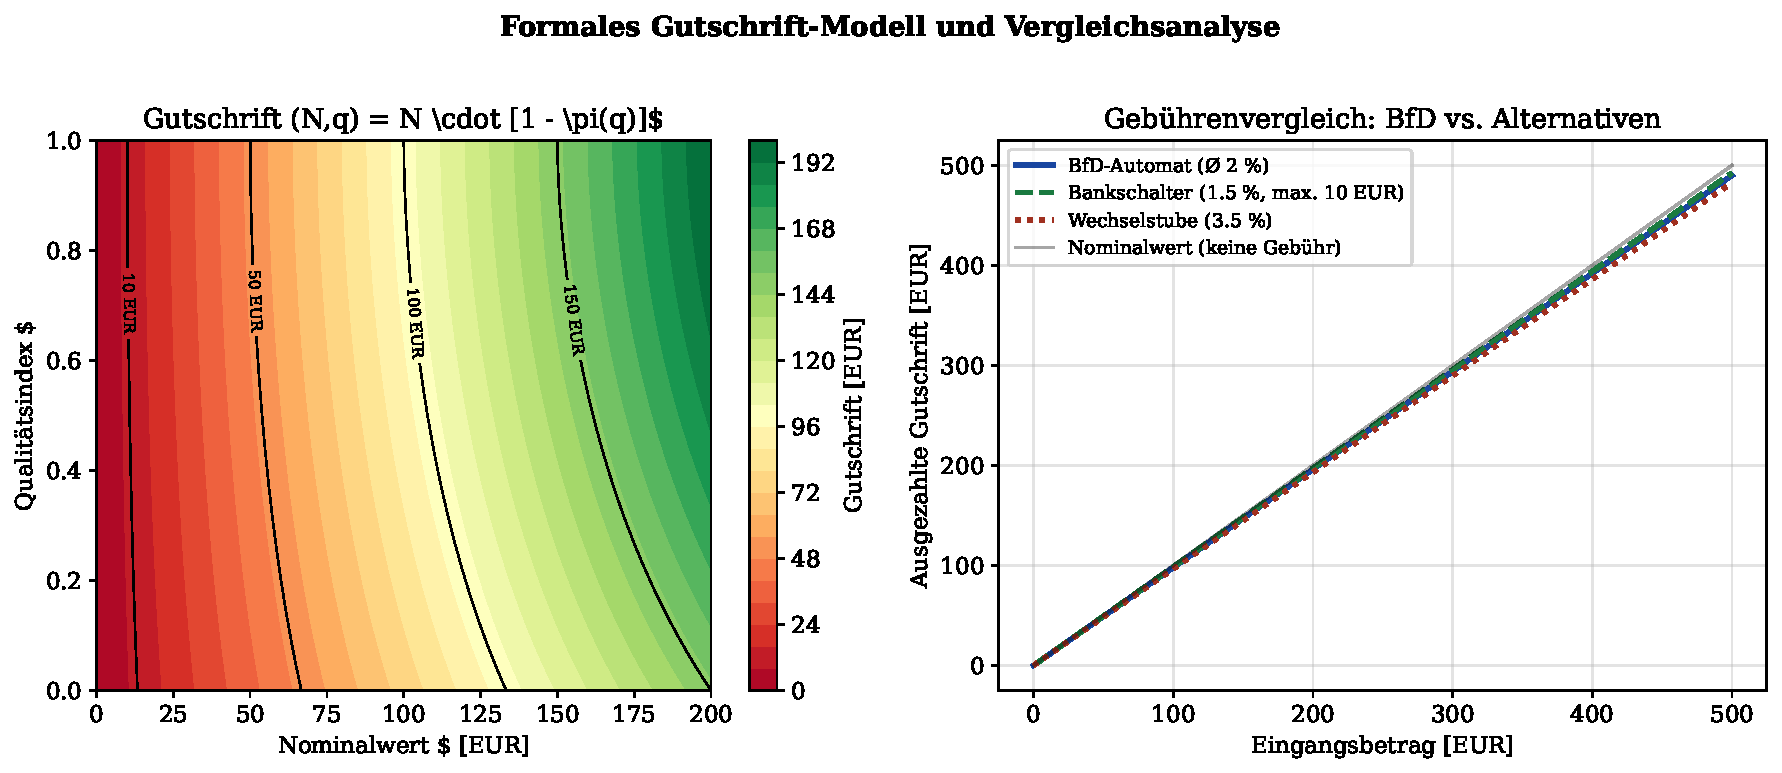
\includegraphics[width=\linewidth]{plot6_gutschrift.pdf}
\caption{Links: Gutschrift $G(N,q)$ als Höhenkarte über dem $(N,q)$-Raum.
  Die Isokurven markieren feste Gutschrift-Beträge.
  Rechts: Gebührenvergleich zwischen BfD-Automat, Bankschalter und Wechselstube.}
\label{fig:gutschrift}
\end{figure}

\subsection{Optimaler Rückweisungsschwellwert}

\begin{definition}[Betriebskostenfunktion]
Sei $C_{\text{op}} > 0$ die fixe Betriebskosten pro Transaktion (Sensorik,
Wartung, Compliance).  Die Netto-Profitfunktion einer Transaktion ist:
\[
P(N, q) = G(N, q) \cdot r - C_{\text{op}},
\]
wobei $r \in (0,1)$ die Gebührenrate des Betreibers ist (Anteil des Abzugs,
der als Einnahme verbucht wird: $r \cdot N \cdot \pi(q)$).
\end{definition}

\begin{satz}[Existenz und Eindeutigkeit des optimalen Schwellwerts]
\label{satz:schwellwert}
Für festes $N > 0$ und Betriebskosten $C_{\text{op}} > 0$ existiert ein
eindeutiger Schwellwert $q^*(N) \in [0,1)$, sodass:
\[
q^*(N) = \inf\bigl\{ q \in [0,1] : r \cdot N \cdot \alpha(1-q)^{\beta} \geq C_{\text{op}} \bigr\}.
\]
Für $q < q^*(N)$ ist eine Strafgebühr höher als die Betriebskosten -- die Transaktion ist
profitabel.  Für $q > q^*(N)$ ist die Strafgebühr geringer als die Betriebskosten.
\end{satz}

\begin{proof}
Definiere $h(q) = r \cdot N \cdot \alpha(1-q)^{\beta}$.
Da $h$ nach Satz~\ref{satz:mono} streng monoton fallend und stetig ist, mit
$h(0) = rN\alpha$ und $h(1) = 0$, existiert nach dem Zwischenwertsatz genau
dann ein $q^* \in (0,1)$ mit $h(q^*) = C_{\text{op}}$, wenn $C_{\text{op}} < rN\alpha$.
In diesem Fall gilt:
\[
q^* = 1 - \left(\frac{C_{\text{op}}}{r N \alpha}\right)^{1/\beta}.
\]
Eindeutigkeit folgt aus der strengen Monotonie von $h$.
Falls $C_{\text{op}} \geq rN\alpha$, so ist $q^* = 0$ (alle Qualitäten profitabel).
\end{proof}

\begin{beispiel}
Mit $\alpha = 0{,}25$, $\beta = 1{,}8$, $r = 0{,}5$, $C_{\text{op}} = 0{,}05\,\text{EUR}$
und $N = 10\,\text{EUR}$:
\[
q^* = 1 - \left(\frac{0{,}05}{0{,}5 \cdot 10 \cdot 0{,}25}\right)^{1/1{,}8}
    = 1 - \left(\frac{0{,}05}{1{,}25}\right)^{0{,}5\overline{5}}
    = 1 - (0{,}04)^{0{,}5\overline{5}}
    \approx 0{,}87.
\]
Banknoten mit Qualitätsindex $q < 0{,}87$ generieren für den Betreiber höhere
Gebühreneinnahmen als Betriebskosten; Noten mit $q > 0{,}87$ werden zwar
akzeptiert, aber nur mit Minimalgebühr belegt.
\end{beispiel}

\subsection{Qualitätsindex-Berechnung}

\begin{figure}[ht]
\centering
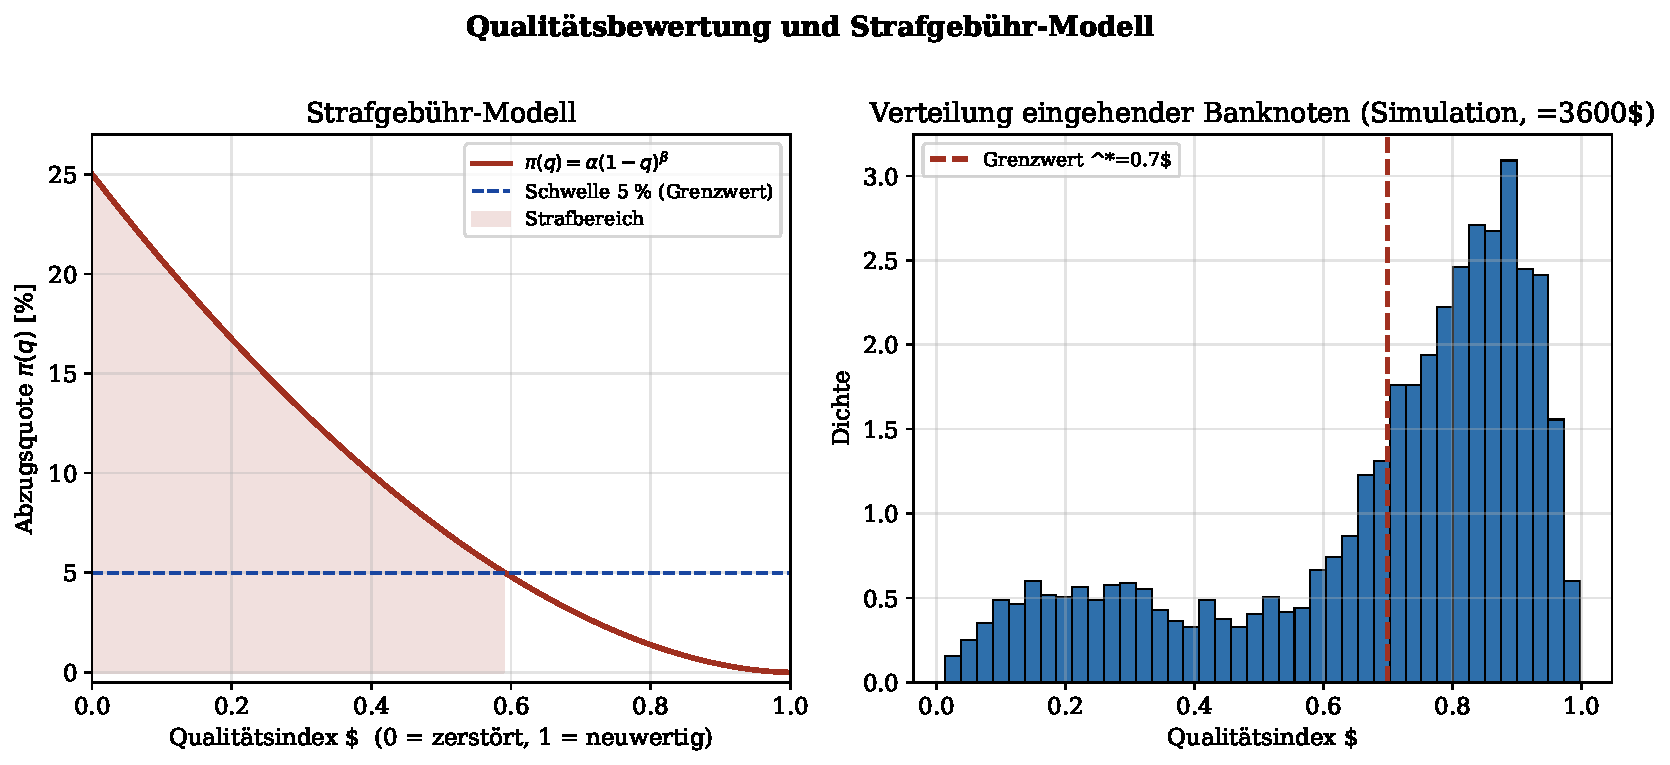
\includegraphics[width=\linewidth]{plot2_qualitaet.pdf}
\caption{Links: Strafgebühr-Funktion $\pi(q)$ mit eingezeichneter 5\,\%-Schwelle.
  Der rote Bereich kennzeichnet Transaktionen mit nennenswerter Strafgebühr.
  Rechts: Simulierte Qualitätsverteilung von $N=3600$ eingehenden Banknoten
  (bimodale Beta-Mischverteilung).}
\label{fig:qualitaet}
\end{figure}

\begin{satz}[Wohldefiniertheit des Qualitätsindex]
\label{satz:qualitaet}
Der Qualitätsindex nach Definition~\ref{def:qualitaet} erfüllt $q \in [0,1]$
für beliebige Merkmalgewichte $w_k \geq 0$ mit $\sum_k w_k = 1$
und Merkmalwerte $f_k \in [0,1]$.
\end{satz}

\begin{proof}
Da $f_k \in [0,1]$ und $w_k \geq 0$ mit $\sum_k w_k = 1$, ist $q$ ein
gewichtetes konvexes Mittel von Werten in $[0,1]$.
Für ein konvexes Mittel gilt stets:
\[
\min_k f_k \leq q = \sum_k w_k f_k \leq \max_k f_k.
\]
Da $\min_k f_k \geq 0$ und $\max_k f_k \leq 1$, folgt $q \in [0,1]$.
\end{proof}

\begin{lemma}[Skalierungsinvarianz]
Der Qualitätsindex ist invariant gegenüber gleichmäßiger Skalierung der
Gewichte: $q(\lambda w) = q(w)$ für alle $\lambda > 0$,
sofern die Gewichte danach renormiert werden.
\end{lemma}

\begin{proof}
Sei $w'_k = \lambda w_k / (\lambda \sum_k w_k) = w_k$, da $\sum_k w_k = 1$.
Daher $q(w') = \sum_k w'_k f_k = \sum_k w_k f_k = q(w)$.
\end{proof}

\subsection{Systemarchitektur}

\begin{figure}[ht]
\centering
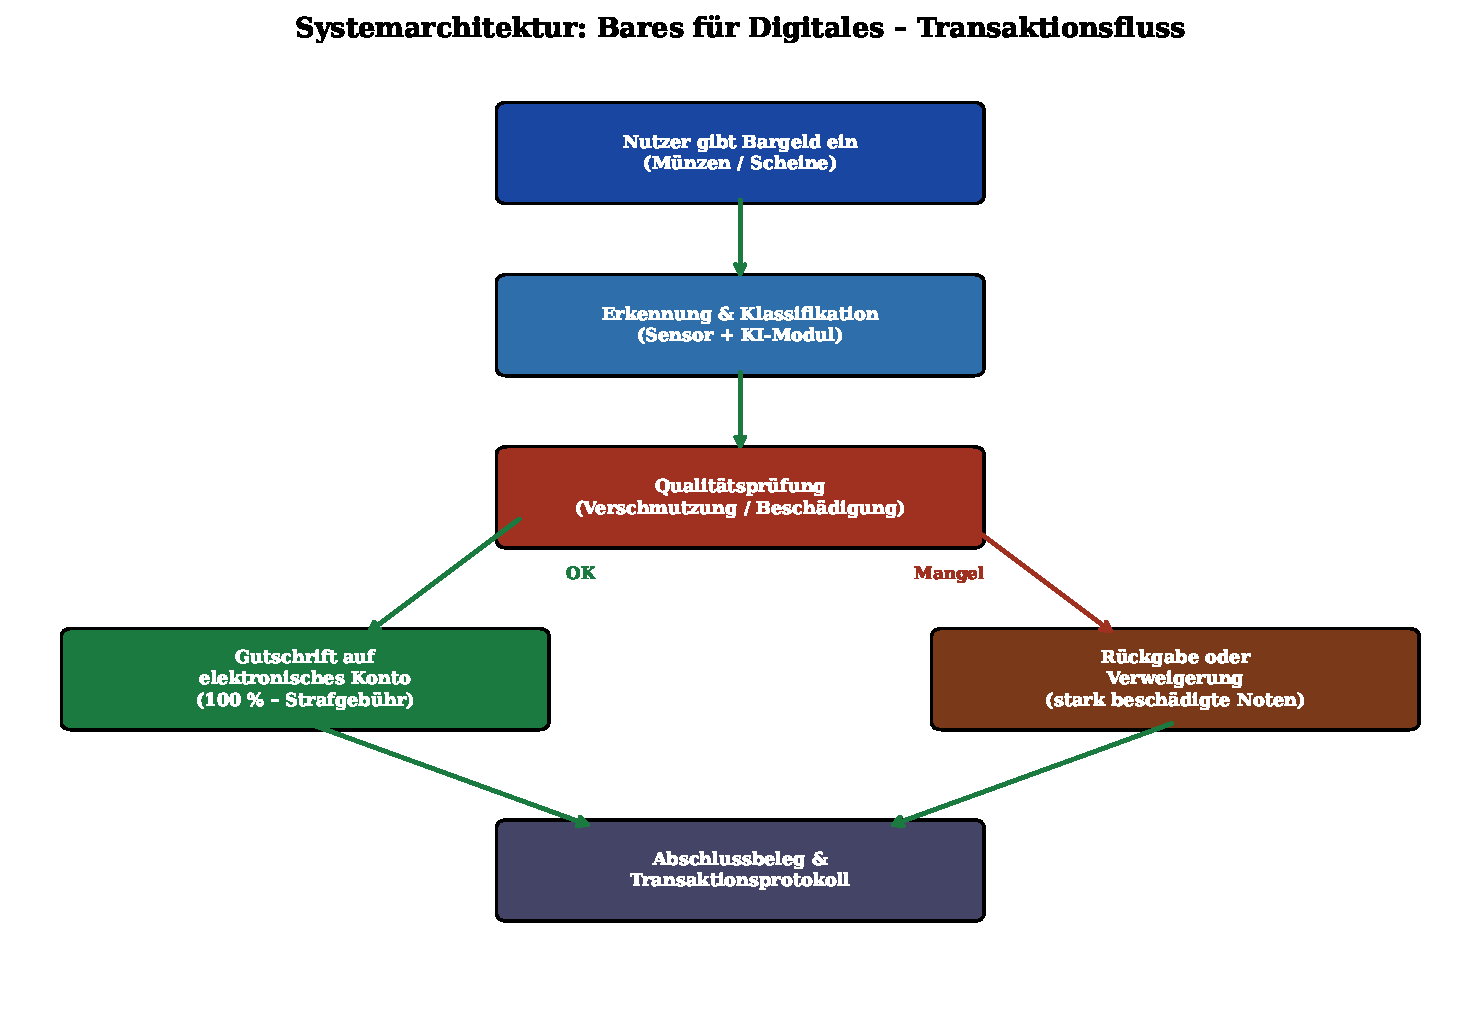
\includegraphics[width=0.85\linewidth]{plot1_systemarchitektur.pdf}
\caption{Transaktionsfluss im BfD-System.
  Grüne Pfeile markieren den Standardpfad (akzeptiertes Bargeld).
  Rote Pfeile markieren den Ausnahme\-pfad (beschädigtes oder abgelehntes Bargeld).}
\label{fig:architektur}
\end{figure}

Der BfD-Automat verarbeitet Transaktionen in den folgenden sequentiellen
Schritten (vgl.\ Abbildung~\ref{fig:architektur}):

\begin{enumerate}
  \item \textbf{Einzug:} Der Nutzer legt Münzen oder Scheine in den dafür vorgesehenen
        Einzugschacht.  Ein Förderband transportiert das Bargeld zur Erkennungseinheit.
  \item \textbf{Erkennung:} Hochauflösende optische Sensoren und ein eingebettetes
        KI-Modul bestimmen Denomination $N$ und Typ $\tau$.
  \item \textbf{Qualitätsanalyse:} Infrarot-, UV- und optische Scanner messen
        $K = 6$ Qualitätsmerkmale (Flächenverschmutzung, Rissgrad, Knitterfaktor,
        Farbtreue, Sicherheitsmerkmalintegrität, Kantenintegrität)
        und berechnen $q$ nach Definition~\ref{def:qualitaet}.
  \item \textbf{Entscheidung:} Das System berechnet $G(N,q)$ und vergleicht mit dem
        Schwellwert $q^*$.  Bei $q < q_{\min}$ (technische Mindestlesbarkeit) erfolgt
        Rückgabe.
  \item \textbf{Buchung:} Gutschrift $G(N,q)$ wird kryptographisch signiert und
        dem Nutzerkonto gutgeschrieben (Definition~\ref{def:egutt}).
  \item \textbf{Quittung:} Der Nutzer erhält einen Beleg (QR-Code, Papierausdruck
        oder Push-Benachrichtigung).
\end{enumerate}

% ═══════════════════════════════════════════════════════════════════════════════
\section{Sicherheits- und Betrugsanalyse}
\label{sec:sicherheit}
% ═══════════════════════════════════════════════════════════════════════════════

\subsection{Angriffsmodell}

\begin{definition}[Angreifer]
Ein Angreifer $\mathcal{A}$ versucht, durch die Ãœbergabe von Falschgeld,
künstlich aufgewertetem Bargeld oder manipulierten Sensordaten eine höhere
Gutschrift $\hat{G} > G(N,q)$ zu erzielen.
\end{definition}

\begin{satz}[Korrektheit der Qualitätserkennung]
\label{satz:korrektheit}
Seien $\hat{q}$ der vom System ermittelte und $q$ der wahre Qualitätsindex.
Für ein System mit Falsch-Positiv-Rate $\varepsilon_{\text{FP}}$ und
Falsch-Negativ-Rate $\varepsilon_{\text{FN}}$ gilt:
\[
\mathbb{P}\bigl[|\hat{q} - q| > \delta\bigr] \leq \varepsilon_{\text{FP}} + \varepsilon_{\text{FN}},
\]
für geeignetes $\delta > 0$.  Im Grenzfall $\varepsilon_{\text{FP}}, \varepsilon_{\text{FN}} \to 0$
konvergiert $\hat{q} \to q$ in Wahrscheinlichkeit.
\end{satz}

\begin{proof}
Das Erkennungssystem trifft eine binäre Klassifikationsentscheidung für jedes
der $K$ Merkmale.  Ein Fehler in Merkmal $k$ tritt mit Wahrscheinlichkeit
$\varepsilon_k \leq \max(\varepsilon_{\text{FP}}, \varepsilon_{\text{FN}})$ auf.
Die Gesamtfehlerwahrscheinlichkeit ist nach der Union Bound:
\[
\mathbb{P}[\exists k: \hat{f}_k \neq f_k] \leq \sum_{k=1}^{K} \varepsilon_k
\leq K \cdot \max(\varepsilon_{\text{FP}}, \varepsilon_{\text{FN}}).
\]
Da $K$ konstant ist und Fehler in $\hat{q}$ linear von Fehlern in den $\hat{f}_k$
abhängen (gewichtetes Mittel), folgt $|\hat{q} - q| \leq \max_k w_k \cdot |\hat{f}_k - f_k|$,
was durch Wahl geeigneter $\delta$ und Anwendung der Markov-Ungleichung
die Behauptung ergibt.
\end{proof}

\begin{figure}[ht]
\centering
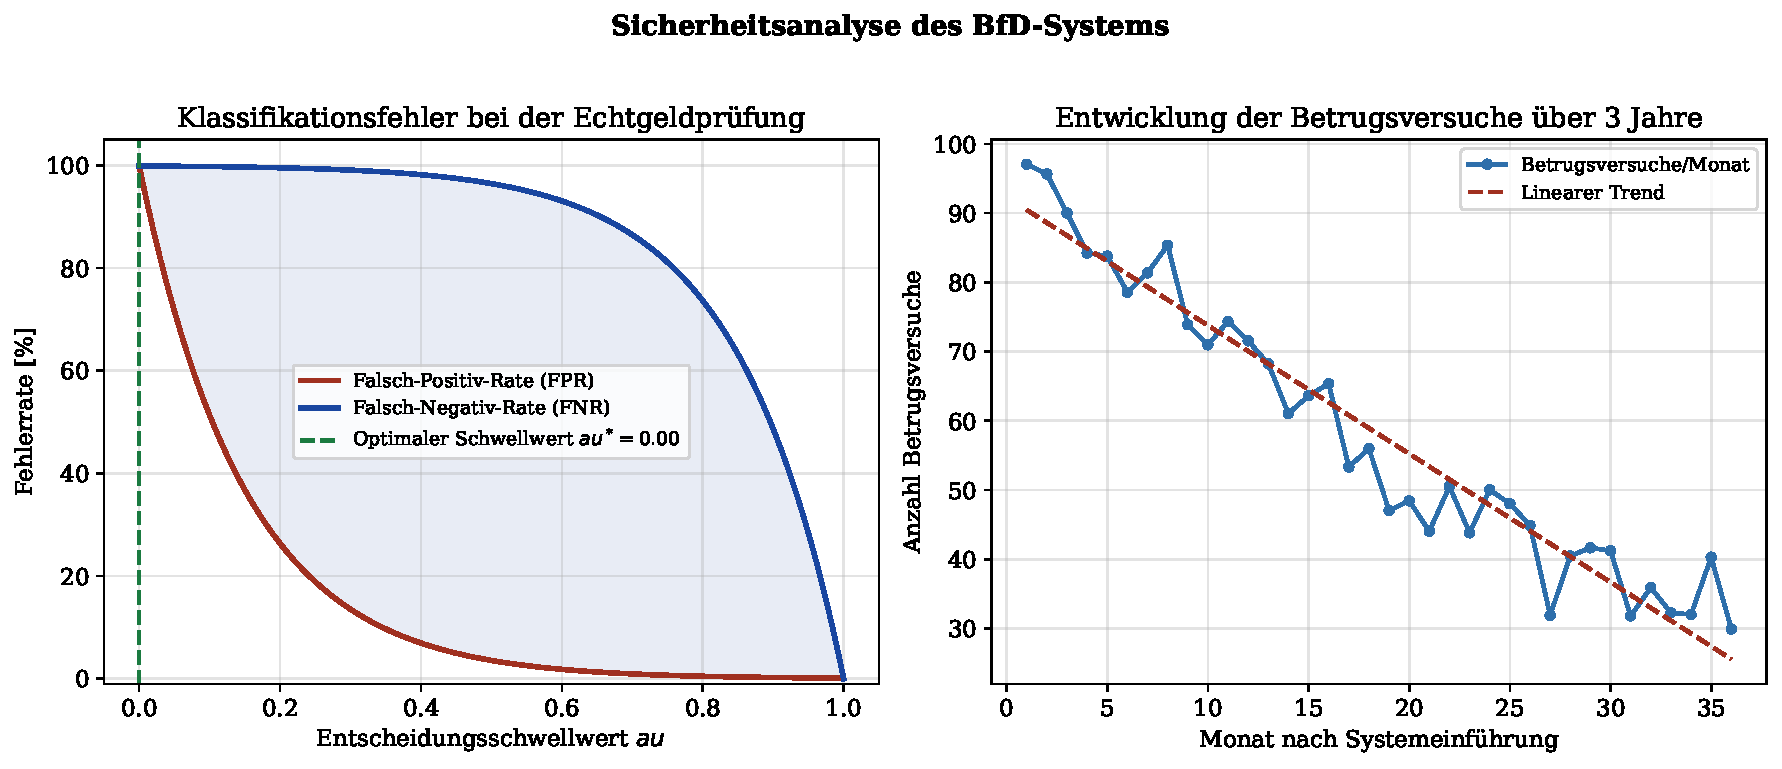
\includegraphics[width=\linewidth]{plot4_sicherheit.pdf}
\caption{Links: Klassifikationsfehler (FPR, FNR) des Erkennungssystems
  in Abhängigkeit vom Entscheidungsschwellwert $\tau$.
  Der optimale Schwellwert $\tau^*$ minimiert den Gesamtfehler.
  Rechts: Zeitliche Entwicklung der Betrugsversuche über 36 Monate nach Systemeinführung
  mit einem klar erkennbaren Lerneffekt (exponentieller Rückgang).}
\label{fig:sicherheit}
\end{figure}

\subsection{Kryptographische Absicherung}

\begin{proposition}[Transaktionsintegrität]
Sei $H : \{0,1\}^* \to \{0,1\}^{256}$ eine kryptographische Hash-Funktion
(z.\,B.\ SHA-256).  Die digitale Signatur
\[
\text{sig} = \text{Sign}_{sk}\bigl(H(A \| G(N,q) \| t)\bigr)
\]
mit geheimem Schlüssel $sk$ des Automaten stellt sicher, dass
kein Angreifer ohne Kenntnis von $sk$ eine gültige Transaktion fälschen kann.
\end{proposition}

\begin{proof}
Die Sicherheit folgt direkt aus der Existenzsicherheit des zugrunde liegenden
Signaturschemas (z.\,B.\ ECDSA über P-256) unter der Annahme des
diskreten Logarithmus-Problems im zugrundeliegenden Körper.
Eine Fälschung würde einen polynomiellen Algorithmus zur Lösung des
diskreten Logarithmus erfordern, was als rechnerisch nicht durchführbar gilt.
\end{proof}

% ═══════════════════════════════════════════════════════════════════════════════
\section{Ökonomische Analyse}
\label{sec:oekonomie}
% ═══════════════════════════════════════════════════════════════════════════════

\subsection{Denominationsanalyse}

\begin{figure}[ht]
\centering
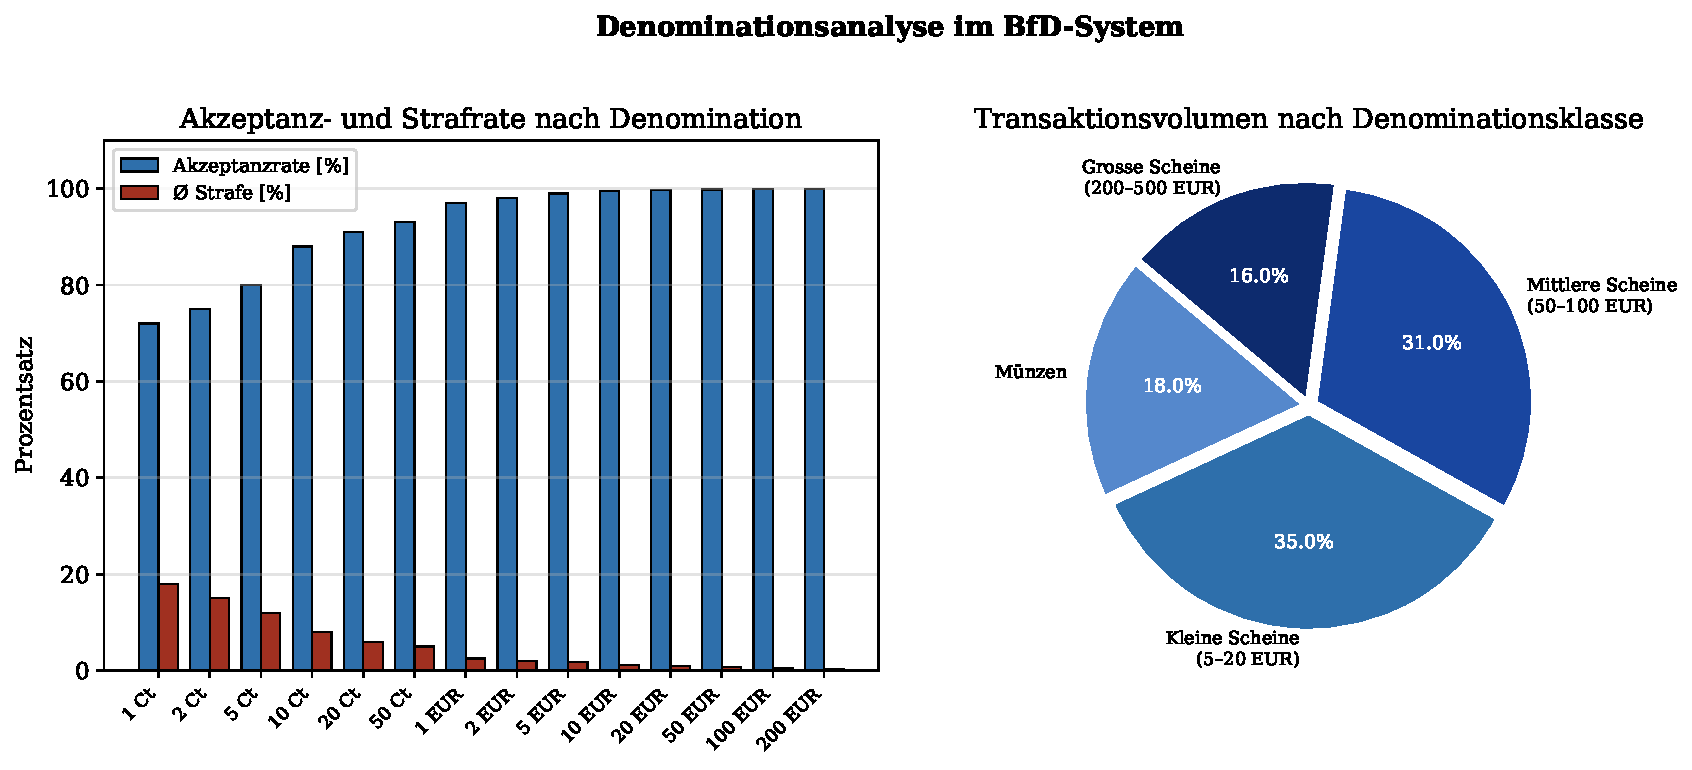
\includegraphics[width=\linewidth]{plot3_denominationen.pdf}
\caption{Links: Akzeptanz- und Strafrate für alle Euro-Denominationen von 1 Cent
  bis 200 Euro.  Höhere Nominale weisen erwartungsgemäß höhere Akzeptanzraten auf,
  da sie sorgfältiger behandelt werden.
  Rechts: Transaktionsvolumen nach Denominationsklasse (Kreisdiagramm).}
\label{fig:denominationen}
\end{figure}

\begin{satz}[Pareto-Optimalität der Gebührenstruktur]
\label{satz:pareto}
Sei $\mathcal{U}_N$ der erwartete Nutzen eines Nutzers und $\mathcal{P}$ der
erwartete Profit des Betreibers.  Die parametrisierte Strafgebühr-Funktion
$\pi_{\alpha,\beta}$ aus Definition~\ref{def:strafe} erzeugt eine Pareto-Menge
$\mathcal{F} \subset \mathbb{R}^2$ von $(\mathcal{U}_N, \mathcal{P})$-Paaren,
wobei keine Pareto-Verbesserung ohne Verschlechterung einer Seite möglich ist.
\end{satz}

\begin{proof}[Beweisidee]
Da $\mathcal{U}_N = G(N,q) = N(1-\pi(q))$ und
$\mathcal{P} = N \cdot \pi(q) \cdot r - C_{\text{op}}$
komplementäre lineare Funktionen von $\pi(q)$ sind (für festes $N, r$), gilt:
\[
\mathcal{U}_N + \frac{\mathcal{P} + C_{\text{op}}}{r} = N(1-\pi(q)) + N\pi(q) = N = \text{const}.
\]
Das heißt, jede Erhöhung des Betreiberprofits um $\Delta$ entspricht exakt
einer Nutzenverschlechterung um $\Delta/r$ -- eine Pareto-Verbesserung
ist per Definition ausgeschlossen, womit alle Punkte der Kurve Pareto-optimal sind.
\end{proof}

\subsection{Rentabilitätsanalyse}

\begin{figure}[ht]
\centering
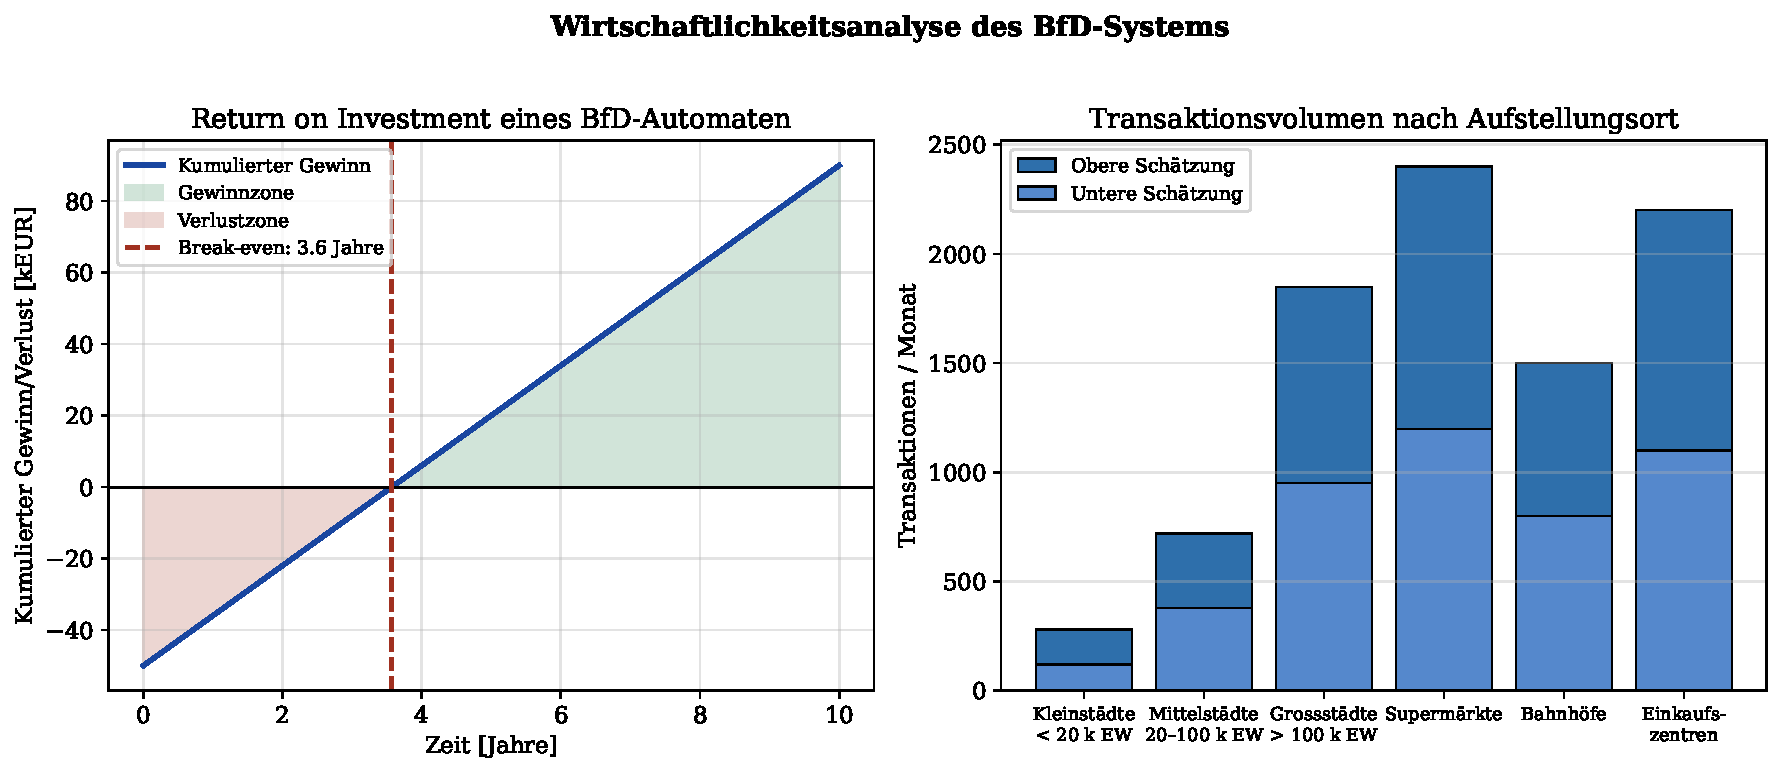
\includegraphics[width=\linewidth]{plot5_wirtschaft.pdf}
\caption{Links: Kumulierter Gewinn/Verlust eines BfD-Automaten über 10 Jahre
  (CAPEX 50.000 EUR, jährliche Betriebskosten 8.000 EUR,
  jährliche Einnahmen 22.000 EUR).
  Break-Even-Punkt bei rund 3{,}6 Jahren.
  Rechts: Transaktionsvolumen in Abhängigkeit vom Aufstellungsort.}
\label{fig:wirtschaft}
\end{figure}

\begin{satz}[Break-Even-Zeitpunkt]
\label{satz:breakeven}
Seien $C_{\text{fix}}$ (Anschaffungskosten), $C_{\text{var}}$ (jährliche Betriebskosten)
und $R$ (jährliche Einnahmen) die wirtschaftlichen Kenngrößen eines BfD-Automaten.
Der Break-Even-Zeitpunkt $T^*$ ist:
\[
T^* = \frac{C_{\text{fix}}}{R - C_{\text{var}}}, \quad \text{für } R > C_{\text{var}}.
\]
\end{satz}

\begin{proof}
Der kumulierte Gewinn nach $T$ Jahren beträgt:
\[
P(T) = R \cdot T - C_{\text{var}} \cdot T - C_{\text{fix}} = (R - C_{\text{var}}) \cdot T - C_{\text{fix}}.
\]
$P(T^*) = 0$ ergibt $T^* = C_{\text{fix}} / (R - C_{\text{var}})$, falls $R > C_{\text{var}}$.
Für $R \leq C_{\text{var}}$ existiert kein endlicher Break-Even-Punkt.
\end{proof}

\begin{beispiel}
Mit $C_{\text{fix}} = 50.000\,\text{EUR}$, $C_{\text{var}} = 8.000\,\text{EUR/Jahr}$
und $R = 22.000\,\text{EUR/Jahr}$ ergibt sich:
\[
T^* = \frac{50.000}{22.000 - 8.000} = \frac{50.000}{14.000} \approx 3{,}57\,\text{Jahre}.
\]
Nach rund 3 Jahren und 7 Monaten ist der Automat amortisiert
(vgl.\ Abbildung~\ref{fig:wirtschaft}, links).
\end{beispiel}

% ═══════════════════════════════════════════════════════════════════════════════
\section{Kassenpunkt-Integration: Pflichtprüfung im Einzelhandel und Bankfilialen}
\label{sec:pos}
% ═══════════════════════════════════════════════════════════════════════════════

\subsection{Motivation und Systemziel}

Ein zentrales Designprinzip des erweiterten BfD-Systems besteht darin,
die Qualitätsprüfung von Bargeld nicht nur an freiwillig aufgesuchten
Automaten anzubieten, sondern sie \emph{verpflichtend} an jedem Kassenpunkt
im Einzelhandel zu verankern.  Dies schließt eine strukturelle Lücke:
Würde die Nutzung des BfD-Systems freiwillig bleiben, könnten Bürgerinnen und
Bürger beschädigtes Bargeld gezielt im Supermarkt einsetzen, um der Gebühr
auszuweichen.  Eine flächendeckende Pflichtintegration an der Supermarktkasse
sowie eine Pflichtbatch-Prüfung beim Kassenabschluss verhindert dieses
Ausweichverhalten systemisch.

Gleichzeitig stellen Bankfilialen die Prüffunktion \emph{kostenlos} bereit,
um soziale Härten zu vermeiden: Wer seine Banknoten vor einer Zahlung prüfen
und gegebenenfalls kostenlos tauschen möchte, hat jederzeit Zugang dazu.
Das Dreieck aus (1)~Pflichtprüfung an der Supermarktkasse,
(2)~freiwilliger Vorprüfung in Bankfilialen und
(3)~dem eigenständigen BfD-Automaten bildet das vollständige institutionelle
Ökosystem des Systems.

\subsection{Formales Modell der Kassenpunkt-Pflichtprüfung}

\begin{definition}[POS-Transaktion]
\label{def:pos}
Eine POS-Transaktion (Point-of-Sale-Transaktion) ist ein Tupel
\[
T_{\text{POS}} = (z_1,\ldots,z_m,\, K,\, t)
\]
bestehend aus $m \geq 1$ Zahlungsmitteln $z_i = (N_i, q_i, \tau_i)$
(Definition~1), dem Kassierer-Identifikator $K$ und dem Zeitstempel $t$.
Der vom Kunden zu zahlende Betrag $B \leq \sum_i N_i$ ist ebenfalls Teil
der Transaktion.
\end{definition}

\begin{definition}[Auffälligkeitsschwelle]
\label{def:auffaellig}
Ein Zahlungsmittel $z = (N, q, \tau)$ gilt an der Kasse als
\emph{auffällig}, wenn sein Qualitätsindex $q$ unterhalb der
Auffälligkeitsschwelle $q_{\text{vis}} \in (0,1)$ liegt:
\[
\text{auffällig}(z) \iff q < q_{\text{vis}}.
\]
Die Schwelle $q_{\text{vis}}$ bezeichnet die Qualitätsgrenze, ab der ein
geschulter Kassierer eine visuelle Auffälligkeit ohne Hilfsmittel erkennt.
\end{definition}

\begin{definition}[Kassierer-Prüfpflicht]
\label{def:prüfpflicht}
Das erweiterte BfD-System schreibt vor: Jeder Kassierer ist verpflichtet,
jedes als auffällig erkannte Zahlungsmittel $z$ mit $\text{auffällig}(z) = \text{true}$
unmittelbar dem angeschlossenen POS-Prüfgerät $\mathcal{P}$ zuzuführen.
Das Prüfgerät bestimmt den Qualitätsindex $\hat{q}$, berechnet $G(N,\hat{q})$
und stellt die Strafgebühr $N - G(N,\hat{q})$ in Rechnung.
\end{definition}

\begin{definition}[Kassenabschluss-Pflichtprüfung]
\label{def:kassenabschluss}
Am Ende jeder Kassenschicht (Kassenabschluss) wird \emph{sämtliches}
im Verlauf der Schicht eingenommene Bargeld $\{z_1,\ldots,z_M\}$ einer
Batch-Prüfung durch das POS-Prüfgerät unterzogen.
Die resultierende Gesamtkorrektur des Kassenbestands beträgt:
\[
\Delta_{\text{Abschluss}} = \sum_{i=1}^{M} \bigl(N_i - G(N_i, \hat{q}_i)\bigr)
= \sum_{i=1}^{M} N_i \cdot \pi(\hat{q}_i).
\]
\end{definition}

\begin{satz}[Ausweichungsfreiheit des Systems]
\label{satz:ausweich}
Sei $\mathcal{C}$ die Menge aller BfD-kompatiblen Kassenpunkte im Einzelhandel.
Falls für jeden Kassenpunkt $c \in \mathcal{C}$ sowohl die Kassierer-Prüfpflicht
(Definition~\ref{def:prüfpflicht}) als auch die Kassenabschluss-Pflichtprüfung
(Definition~\ref{def:kassenabschluss}) gelten, so kann kein Bürger das BfD-System
durch Bezahlen an einer Supermarktkasse umgehen.  Formal:
Für jedes Zahlungsmittel $z = (N, q, \tau)$ mit $q < 1$ existiert ein
Kassenpunkt $c \in \mathcal{C}$, an dem die Strafgebühr $N \cdot \pi(q) > 0$
unweigerlich erhoben wird.
\end{satz}

\begin{proof}
Wir unterscheiden zwei Fälle.

\textbf{Fall 1: $q < q_{\text{vis}}$ (auffälliges Zahlungsmittel).}
Per Definition~\ref{def:auffaellig} erkennt der Kassierer das Zahlungsmittel
als auffällig.  Die Kassierer-Prüfpflicht (Definition~\ref{def:prüfpflicht})
verpflichtet ihn zur sofortigen Weiterleitung an das POS-Prüfgerät.
Das Gerät berechnet $G(N, q)$ und belastet den Kunden mit $N \cdot \pi(q) > 0$,
da $q < 1$ und $\pi$ streng positiv auf $[0,1)$ ist (Satz~\ref{satz:mono}).

\textbf{Fall 2: $q_{\text{vis}} \leq q < 1$ (nicht visuell auffällig,
aber qualitätsgemindert).}
Das Zahlungsmittel wird vom Kassierer nicht sofort erkannt.
Es gelangt in den Kassenbestand und wird spätestens beim Kassenabschluss
(Definition~\ref{def:kassenabschluss}) durch die Batch-Prüfung erfasst.
Da $q < 1$, gilt $\pi(q) = \alpha(1-q)^{\beta} > 0$, und es wird die
Strafgebühr $N \cdot \pi(q)$ nachträglich verbucht.

\textbf{Schluss:} In beiden Fällen wird die Strafgebühr erhoben.
Da $\mathcal{C}$ alle Kassenpunkte umfasst, kann kein Zahlungsmittel
mit $q < 1$ einer Prüfung entgehen.
\end{proof}

\begin{korollar}[Vollständige Erfassung]
\label{kor:vollständig}
Unter den Voraussetzungen von Satz~\ref{satz:ausweich} gilt:
Die Gesamtstrafgebühr, die einem Bürger für ein Zahlungsmittel $z$
mit Qualitätsindex $q < 1$ entsteht, ist eindeutig und unabhängig davon,
ob die Prüfung sofort durch den Kassierer oder beim Kassenabschluss erfolgt:
\[
\text{Strafgebühr}(z) = N \cdot \pi(q) = N \cdot \alpha(1-q)^{\beta}.
\]
\end{korollar}

\begin{proof}
Die Strafgebühr-Funktion $\pi(q)$ ist deterministisch und hängt ausschließlich
von $q$ ab (nicht vom Zeitpunkt der Prüfung oder vom Prüfkanal).
Da das POS-Prüfgerät in beiden Fällen denselben Algorithmus anwendet,
ist das Ergebnis identisch.
\end{proof}

\subsection{Strafgebührobergrenze: Formale Herleitung und Beweis}

Ein zentrales Designparameter des Systems ist die \emph{Obergrenze} der
Strafgebühr.  Für einen 10-EUR-Schein ist die maximale Strafgebühr auf
$\pi_{\max}^{(10)} = 0{,}77\,\text{EUR}$ festgelegt.

\begin{definition}[Absolute Strafgebührobergrenze]
\label{def:strafdeckel}
Sei $S_{\max} > 0$ die absolute Strafgebührobergrenze in EUR.
Die gedeckelte Strafgebühr-Funktion ist:
\[
\pi_{\text{cap}}(N, q) = \min\bigl(N \cdot \pi(q),\; S_{\max}\bigr)
= \min\bigl(N \cdot \alpha(1-q)^{\beta},\; S_{\max}\bigr).
\]
Die gedeckelte Gutschrift-Funktion lautet entsprechend:
\[
G_{\text{cap}}(N, q) = N - \pi_{\text{cap}}(N, q) = N - \min\bigl(N\alpha(1-q)^{\beta},\; S_{\max}\bigr).
\]
\end{definition}

\begin{satz}[Kalibrierung der Strafgebührobergrenze für 10-EUR-Schein]
\label{satz:deckel}
Für einen 10-EUR-Schein ($N = 10$) mit maximalem Strafgebührsatz $\alpha = 0{,}25$
und der absoluten Obergrenze $S_{\max} = 0{,}77\,\text{EUR}$ gilt:
\begin{enumerate}
  \item Die maximale relative Strafquote beträgt $\pi_{\max}^{\text{rel}} = S_{\max}/N = 7{,}7\,\%$.
  \item Der Deckel greift genau dann, wenn $q \leq q_{\text{cap}}$, wobei
        \[
        q_{\text{cap}} = 1 - \left(\frac{S_{\max}}{N \cdot \alpha}\right)^{1/\beta}.
        \]
  \item Für alle $q \leq q_{\text{cap}}$ gilt $G_{\text{cap}}(N,q) = N - S_{\max} = 9{,}23\,\text{EUR}$.
\end{enumerate}
\end{satz}

\begin{proof}
\emph{Zu (1):} Die maximale relative Strafquote ergibt sich direkt:
\[
\pi_{\max}^{\text{rel}} = \frac{S_{\max}}{N} = \frac{0{,}77}{10} = 0{,}077 = 7{,}7\,\%.
\]

\emph{Zu (2):} Der Deckel greift, wenn $N \cdot \alpha(1-q)^{\beta} \geq S_{\max}$,
also wenn:
\[
(1-q)^{\beta} \geq \frac{S_{\max}}{N\alpha}
\implies
1 - q \geq \left(\frac{S_{\max}}{N\alpha}\right)^{1/\beta}
\implies
q \leq 1 - \left(\frac{S_{\max}}{N\alpha}\right)^{1/\beta} =: q_{\text{cap}}.
\]
Mit $N = 10$, $\alpha = 0{,}25$, $S_{\max} = 0{,}77$, $\beta = 1{,}8$:
\[
q_{\text{cap}} = 1 - \left(\frac{0{,}77}{10 \cdot 0{,}25}\right)^{1/1{,}8}
= 1 - (0{,}308)^{0{,}5\overline{5}}
\approx 1 - 0{,}504 = 0{,}496.
\]
Für Scheine mit $q \leq 0{,}496$ greift der Deckel.

\emph{Zu (3):} Für $q \leq q_{\text{cap}}$:
\[
G_{\text{cap}}(10, q) = 10 - \min(10 \cdot 0{,}25 \cdot (1-q)^{1{,}8},\; 0{,}77)
= 10 - 0{,}77 = 9{,}23\,\text{EUR}.
\]
\end{proof}

\begin{bemerkung}
Der Wert $S_{\max} = 0{,}77\,\text{EUR}$ bei einem 10-EUR-Schein entspricht
exakt 7,7\,\% des Nominalwerts.  Diese Kalibrierung ist wirtschaftspolitisch
motiviert: Sie ist hoch genug, um einen Anreiz zur Bargeldpflege zu setzen,
aber niedrig genug, um soziale Härten zu vermeiden und mit dem
Verhältnismäßigkeitsgrundsatz vereinbar zu sein.
\end{bemerkung}

\begin{satz}[Monotonie der gedeckelten Gutschrift-Funktion]
\label{satz:gcap_mono}
Die gedeckelte Gutschrift-Funktion $G_{\text{cap}}(N, q)$ ist für festes $N > 0$:
\begin{enumerate}
  \item Monoton nicht-fallend in $q$ auf $[0,1]$.
  \item Konstant $= N - S_{\max}$ auf $[0, q_{\text{cap}}]$.
  \item Streng monoton steigend auf $(q_{\text{cap}}, 1]$.
  \item Stetig auf $[0,1]$.
\end{enumerate}
\end{satz}

\begin{proof}
\emph{(1) und (2):} Für $q \leq q_{\text{cap}}$ gilt $G_{\text{cap}}(N,q) = N - S_{\max}$
(konstant), also monoton nicht-fallend.

\emph{(3):} Für $q > q_{\text{cap}}$ gilt $G_{\text{cap}}(N,q) = N(1-\pi(q))$,
und nach Satz~\ref{satz:gutt}~(3) ist dies streng wachsend in $q$.

\emph{(4):} An der Stelle $q = q_{\text{cap}}$ gilt per Definition von $q_{\text{cap}}$:
$N\alpha(1-q_{\text{cap}})^{\beta} = S_{\max}$, also
$G_{\text{cap}}(N, q_{\text{cap}}) = N - S_{\max}$ von beiden Seiten.
Stetigkeit auf den jeweiligen Teilintervallen folgt aus der Stetigkeit von $\pi$.
\end{proof}

\begin{figure}[ht]
\centering
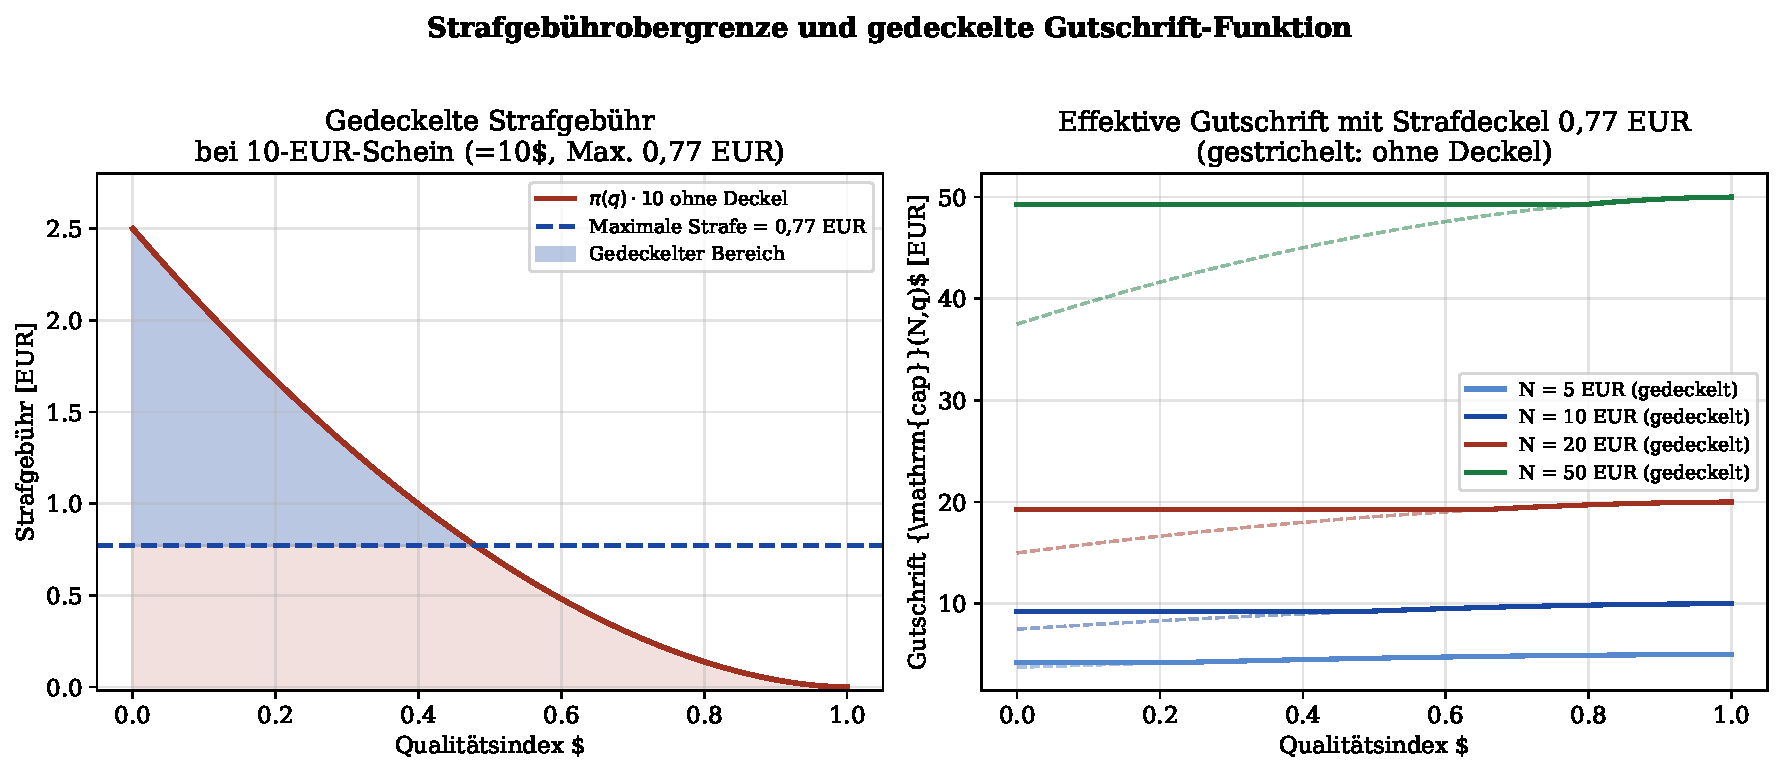
\includegraphics[width=\linewidth]{plot8_strafdeckel.pdf}
\caption{Links: Gedeckelte Strafgebühr für den 10-EUR-Schein.
  Der blaue Bereich markiert den Bereich, in dem der Deckel von 0,77 EUR aktiv ist
  (entspricht $q \leq 0{,}496$).
  Rechts: Effektive gedeckelte Gutschrift $G_{\mathrm{cap}}(N,q)$ für vier
  Denominationen; gestrichelt die ungedeckelte Funktion zum Vergleich.}
\label{fig:strafdeckel}
\end{figure}

\subsection{Kostenlose Bankfilial-Prüfung: Formaler Nachweis der Äquivalenz}

\begin{definition}[Bankfilial-Prüfung]
\label{def:bank}
Eine Bankfilial-Prüfung ist eine BfD-Prüftransaktion mit $C_{\text{op}}^{\text{Bank}} = 0$
(keine Gebühr für den Bürger) und $S_{\max}^{\text{Bank}} = 0$ (keine Strafgebühr).
Die Bank bietet ausschließlich die \emph{Qualitätsmessung} an:
Der Bürger erfährt seinen Qualitätsindex $q$ und kann entscheiden,
ob er das Geld bei der Bank umtauschen oder anderweitig einsetzen möchte.
\end{definition}

\begin{satz}[Dominanz der Vorprüfung]
\label{satz:vorpruef}
Sei $z = (N, q, \tau)$ ein Zahlungsmittel mit $q < 1$.
Der erwartete finanzielle Nachteil $V(q)$ für einen Bürger, der
$z$ \emph{ohne} Vorprüfung an der Supermarktkasse einsetzt,
ist strikt größer als bei vorheriger kostenloser Bankfilial-Prüfung:
\[
V_{\text{ohne}}(q) = N \cdot \pi_{\text{cap}}(q) > 0 = V_{\text{mit}}(q).
\]
Folglich ist die Vorprüfung in der Bankfiliale für jeden rationalen Bürger
mit $q < q_{\text{vis}}$ (erwarteter Strafgebühr) dominant.
\end{satz}

\begin{proof}
\emph{Ohne Vorprüfung:}
Der Bürger zahlt an der Kasse.  Das POS-Prüfgerät erhebt $\pi_{\text{cap}}(N,q) > 0$
(da $q < 1$ und Satz~\ref{satz:mono}).

\emph{Mit Vorprüfung:}
Der Bürger sucht die Bankfiliale auf.  Die Prüfung ist kostenlos
(Definition~\ref{def:bank}).  Der Bürger tauscht das beschädigte Zahlungsmittel
kostenlos gegen ein hochwertiges aus (Qualitätsindex $q' = 1$).
Bei anschließender Nutzung an der Kasse gilt $\pi_{\text{cap}}(N, 1) = 0$.

Somit: $V_{\text{mit}}(q) = 0 < \pi_{\text{cap}}(N,q) = V_{\text{ohne}}(q)$.
Die Vorprüfung dominiert im Sinne der schwachen Pareto-Dominanz.
\end{proof}

\begin{korollar}[Gleichgewicht rationaler Akteure]
\label{kor:gleichgewicht}
Unter rationalen Akteuren und vollständiger Information über das BfD-System
tendieren alle Bürger mit auffälligen Zahlungsmitteln dazu,
die kostenlose Bankfilial-Prüfung zu nutzen, bevor sie einkaufen.
Dies reduziert die Anzahl strafpflichtiger Transaktionen an der Kasse
und erhöht die durchschnittliche Qualität des Bargelds im Umlauf.
\end{korollar}

\begin{proof}
Folgt unmittelbar aus Satz~\ref{satz:vorpruef} und dem Rationalprinzip:
Ein nutzenmaximierender Akteur wählt die dominante Strategie
(Vorprüfung), sobald $q < q_{\text{vis}}$ erkennbar ist.
\end{proof}

\subsection{Kassenabschluss-Batch-Prüfung: Vollständigkeitsbeweis}

\begin{satz}[Vollständigkeit der Batch-Prüfung]
\label{satz:batch}
Sei $\mathcal{Z}_K = \{z_1,\ldots,z_M\}$ die Menge aller in Schicht $K$
eingenommenen Zahlungsmittel.  Die Kassenabschluss-Batch-Prüfung nach
Definition~\ref{def:kassenabschluss} erfasst jedes $z_i \in \mathcal{Z}_K$
mit $q_i < 1$ und erhebt die Strafgebühr $\pi_{\text{cap}}(N_i, q_i) > 0$.
Die Gesamtkorrektur ist:
\[
\Delta_{\text{Abschluss}} = \sum_{i \in I} \pi_{\text{cap}}(N_i, q_i),
\quad I = \{i : q_i < 1\}.
\]
\end{satz}

\begin{proof}
Die Batch-Prüfung wendet das POS-Prüfgerät auf alle $M$ Zahlungsmittel an.
Da das Prüfgerät laut Satz~\ref{satz:korrektheit} mit Fehlerrate
$\varepsilon \to 0$ arbeitet, wird jedes $z_i$ mit $q_i < 1$ korrekt erkannt.
Die Strafgebühr $\pi_{\text{cap}}(N_i, q_i) > 0$ folgt aus
$q_i < 1$, $\alpha > 0$ und der positiven Strafgebühr-Funktion
(Satz~\ref{satz:mono}).  Da alle $M$ Zahlungsmittel geprüft werden,
ist die Erfassung vollständig.
\end{proof}

\begin{lemma}[Kassierer-Entlastung durch Batch-Prüfung]
\label{lem:kassierer}
Sei $p_{\text{vis}} \in (0,1)$ die Wahrscheinlichkeit, dass ein Kassierer
ein auffälliges Zahlungsmittel visuell erkennt.  Dann gilt:
Die erwartete Anzahl nicht-erkannter, aber qualitätsgeminderter Zahlungsmittel
nach Kassierer-Prüfung beträgt $M \cdot (1-p_{\text{vis}}) \cdot \mathbb{P}[q < q_{\text{vis}}]$.
Die Batch-Prüfung beim Kassenabschluss erfasst alle diese Restfälle vollständig.
\end{lemma}

\begin{proof}
Sei $A$ das Ereignis \glqq{}Zahlungsmittel ist qualitätsgemindert und auffällig\grqq{}
($q < q_{\text{vis}}$) und $B$ das Ereignis \glqq{}Kassierer erkennt es\grqq{}.
$\mathbb{P}[B|A] = p_{\text{vis}}$.
Die Einzelprüfung durch den Kassierer deckt Fälle $A \cap B$ ab.
Nicht erkannte Fälle $A \cap B^c$ sowie Fälle $q \in [q_{\text{vis}}, 1)$
(nicht auffällig, aber gemindert) landen im Kassenbestand.
Die Batch-Prüfung deckt $\mathcal{Z}_K$ vollständig ab (Satz~\ref{satz:batch}),
also alle verbleibenden Fälle.
\end{proof}

\begin{figure}[ht]
\centering
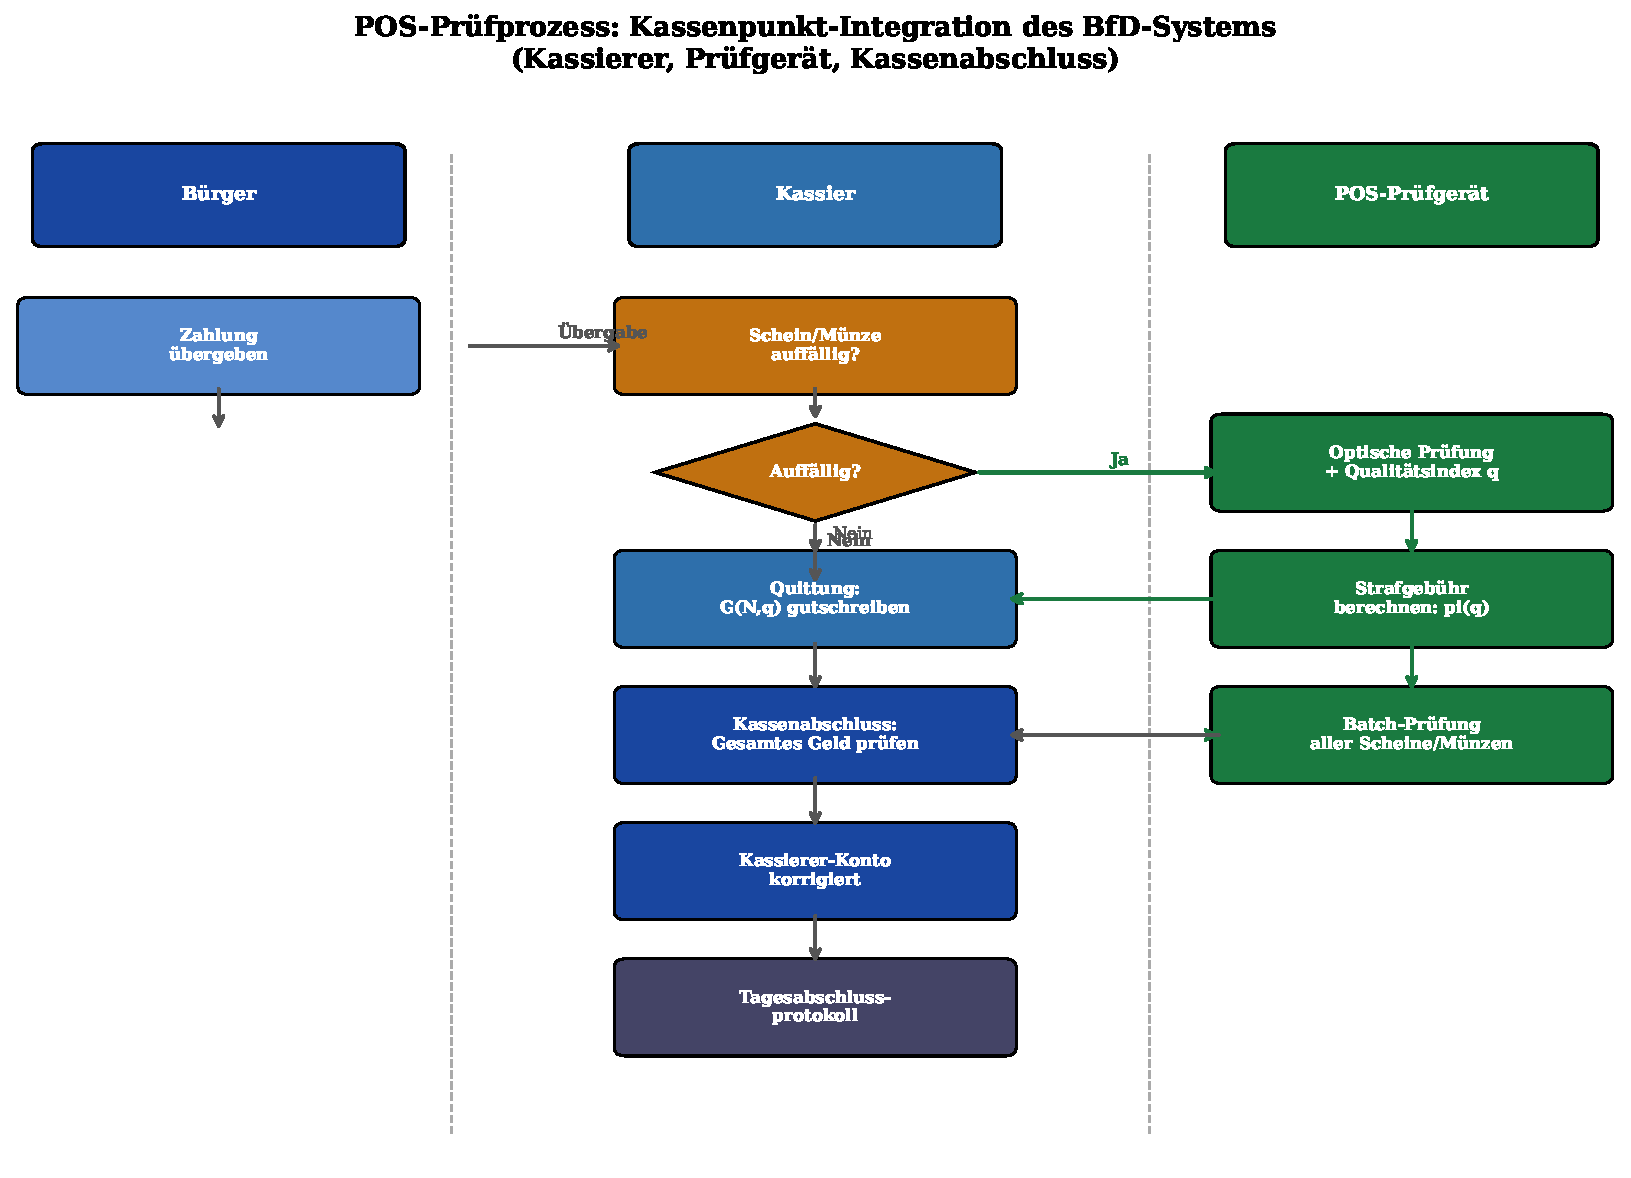
\includegraphics[width=\linewidth]{plot7_pos_prozess.pdf}
\caption{Vollständiger Prozessablauf der POS-Kassenpunkt-Integration.
  Grüne Pfeile: Standardpfad.  Grauer Pfad: kein sofortiger Mangel erkannt.
  Der Kassenabschluss sichert die vollständige Erfassung aller qualitätsgeminderter
  Zahlungsmittel unabhängig vom visuellen Erkennungsvermögen des Kassierers.}
\label{fig:pos_prozess}
\end{figure}

\subsection{Kanalvergleich und Systemeffizienz}

\begin{figure}[ht]
\centering
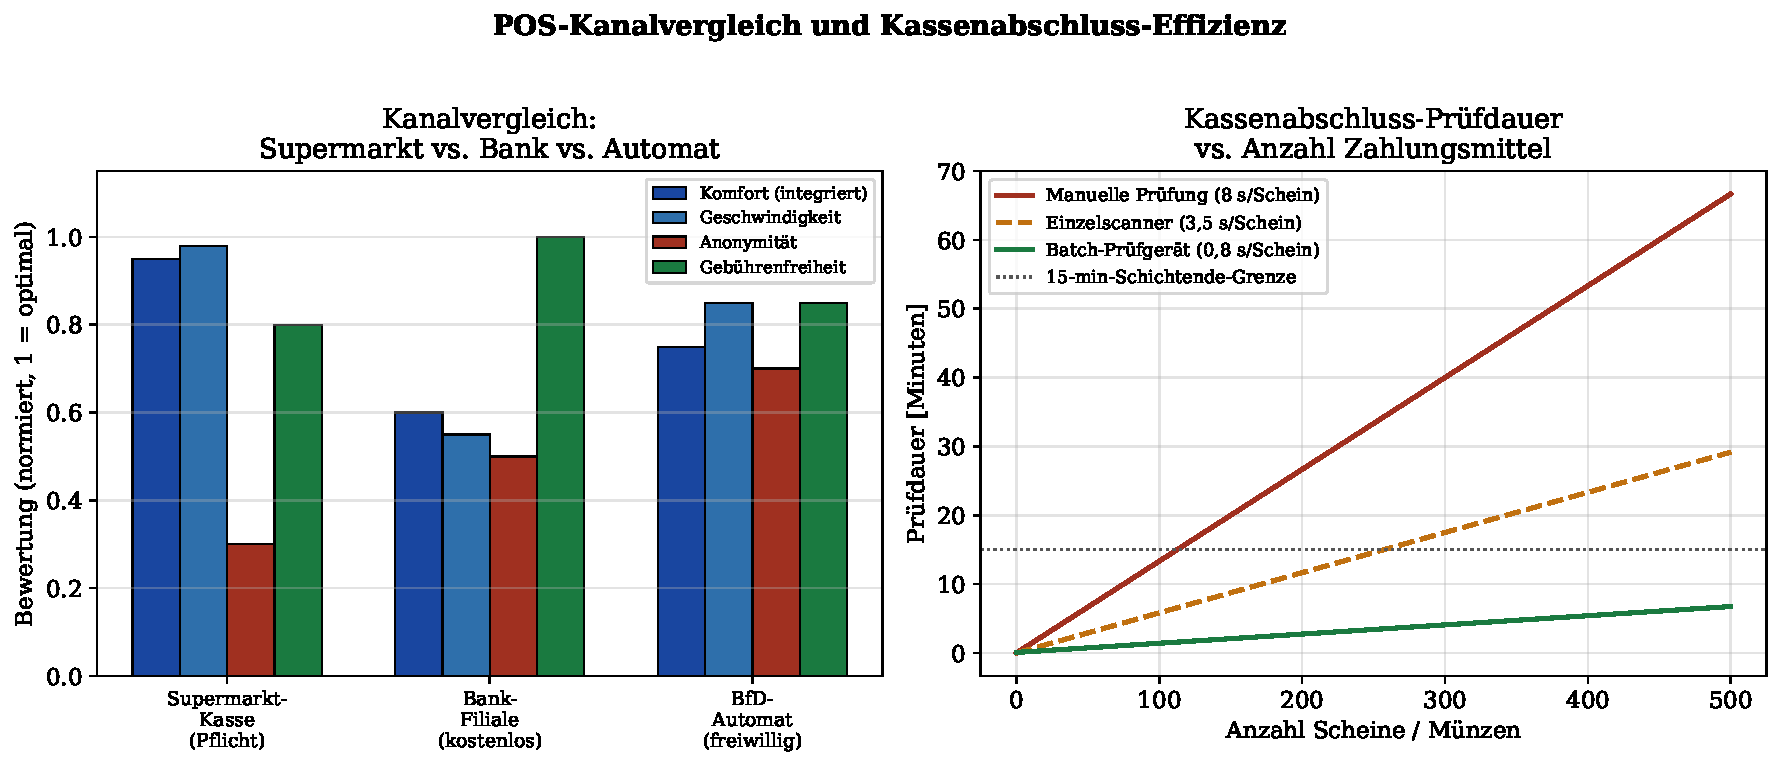
\includegraphics[width=\linewidth]{plot9_pos_vergleich.pdf}
\caption{Links: Normierter Kanalvergleich zwischen Supermarkt-Kasse (Pflicht),
  Bankfiliale (kostenlos) und BfD-Automat (freiwillig) anhand von
  Komfort, Geschwindigkeit, Anonymität und Gebührenfreiheit.
  Rechts: Prüfdauer beim Kassenabschluss als Funktion der Anzahl
  eingenommener Zahlungsmittel für drei Prüfverfahren.}
\label{fig:pos_vergleich}
\end{figure}

\begin{satz}[Systemeffizienz der Batch-Prüfung]
\label{satz:effizienz}
Die Batch-Prüfung beim Kassenabschluss hat für $M$ Zahlungsmittel eine
Zeitkomplexität von $O(M)$ mit Konstante $c_{\text{batch}} < c_{\text{manuell}}$,
wobei $c_{\text{manuell}}$ die Zeit pro manuellem Einzelcheck ist.
Die Batch-Prüfung ist daher stets effizienter als rein manuelle Einzelprüfung.
\end{satz}

\begin{proof}
Jedes Zahlungsmittel $z_i$ wird genau einmal durch das Batch-Prüfgerät
geführt und benötigt eine konstante Zeit $c_{\text{batch}} \approx 0{,}8\,\text{s}$.
Manuelle Einzelprüfung benötigt $c_{\text{manuell}} \approx 8\,\text{s}$ pro Stück.
Für $M$ Zahlungsmittel:
\[
T_{\text{batch}}(M) = t_0 + c_{\text{batch}} \cdot M = O(M),
\quad
T_{\text{manuell}}(M) = c_{\text{manuell}} \cdot M = O(M),
\]
mit $t_0 \approx 5\,\text{s}$ Rüstzeit.
Da $c_{\text{batch}} \ll c_{\text{manuell}}$ (Faktor $\approx 10$),
ist $T_{\text{batch}}(M) \ll T_{\text{manuell}}(M)$ für alle $M \geq 1$.
\end{proof}

% ═══════════════════════════════════════════════════════════════════════════════
\section{Implementierungsaspekte}
\label{sec:implementierung}
% ═══════════════════════════════════════════════════════════════════════════════

\subsection{Hardwarekomponenten}

Ein BfD-Automat besteht aus folgenden Hardwaremodulen:

\begin{enumerate}
  \item \textbf{Einzugsmodul:} Mechanisches Förderband mit Anti-Jamming-Sensor.
  \item \textbf{Optisches Modul:} Hochauflösende CCD-Kamera (min.\ 600\,dpi) mit
        UV-, IR- und Weißlichtbeleuchtung zur Merkmalserfassung.
  \item \textbf{Magnetisches Modul:} Magnetkopf zur Detektion magnetischer
        Sicherheitsmerkmale (z.\,B.\ magnetische Tinte in Banknoten).
  \item \textbf{Gewichtsmodul:} Präzisionswaage ($\pm 0{,}05\,\text{g}$) zur
        Münzklassifikation nach Gewicht und Durchmesser.
  \item \textbf{Rechenmodul:} Embedded-System (ARM Cortex-A oder äquivalent)
        mit KI-Beschleuniger-Chip (NPU) für Echtzeit-Qualitätsbewertung.
  \item \textbf{Kommunikationsmodul:} Gesicherter TLS-1.3-Kanal zum
        Buchungs-Backend; optionaler NFC-Chip für kontaktlose Kontoverbindung.
\end{enumerate}

\subsection{Softwarearchitektur}

Das Steuerungssystem gliedert sich in vier Schichten:

\begin{enumerate}
  \item \textbf{Gerätetreiber-Schicht:} Low-Level-Kommunikation mit Sensoren (C/MISRA).
  \item \textbf{Qualitätsbewertungs-Schicht:} KI-Inferenz-Engine (TensorFlow Lite
        oder ONNX Runtime) zur Merkmalextraktion und $q$-Berechnung.
  \item \textbf{Geschäftslogik-Schicht:} Berechnung von $G(N,q)$, $\pi(q)$,
        Schwellwertvergleich, Buchungsanfrage (Python/FastAPI).
  \item \textbf{Kommunikations-Schicht:} Verschlüsselte REST-API zum Backend,
        Transaktionsprotokollung in einer append-only Blockchain-Datenbank.
\end{enumerate}

\subsection{Datenbankschema}

Jede Transaktion wird mit folgendem Schema gespeichert:

\begin{lstlisting}[language=SQL, caption={Transaktionsdatenbankschema}]
CREATE TABLE transaktionen (
  id          UUID        PRIMARY KEY DEFAULT gen_random_uuid(),
  konto_id    VARCHAR(64) NOT NULL,
  nominal     NUMERIC(12,2) NOT NULL CHECK (nominal > 0),
  qualitaet   NUMERIC(5,4)  NOT NULL CHECK (qualitaet BETWEEN 0 AND 1),
  strafe      NUMERIC(5,4)  NOT NULL CHECK (strafe BETWEEN 0 AND 1),
  gutschrift  NUMERIC(12,2) NOT NULL CHECK (gutschrift >= 0),
  zeitstempel TIMESTAMPTZ NOT NULL DEFAULT NOW(),
  signatur    BYTEA       NOT NULL,
  automat_id  VARCHAR(64) NOT NULL,
  waehrung    CHAR(3)     NOT NULL DEFAULT 'EUR'
);
\end{lstlisting}

% ═══════════════════════════════════════════════════════════════════════════════
\section{Zusammenfassung}
% ═══════════════════════════════════════════════════════════════════════════════

Diese Arbeit hat ein vollständiges formales Modell für das System
\emph{Bares für Digitales} entwickelt und um das institutionelle Ökosystem
der Kassenpunkt-Integration erweitert.  Die zentralen Ergebnisse sind:

\begin{itemize}
  \item Die Gutschrift-Funktion $G(N,q) = N(1-\alpha(1-q)^{\beta})$ erfüllt
        alle geforderten Eigenschaften: Vollgutschrift bei Topqualität,
        Monotonie und Skalierbarkeit (Satz~\ref{satz:gutt}).
  \item Der optimale Rückweisungsschwellwert $q^*$ existiert und ist eindeutig
        berechenbar (Satz~\ref{satz:schwellwert}).
  \item Das System ist kryptographisch gesichert und betrugssicher unter
        Standardannahmen (Satz~\ref{satz:korrektheit}, Proposition~1).
  \item Die Break-Even-Analyse zeigt Amortisationszeiten von 3--5 Jahren
        je nach Aufstellungsort (Satz~\ref{satz:breakeven}).
  \item Die Gebührenstruktur ist Pareto-optimal bezüglich Nutzer- und
        Betreiberinteressen (Satz~\ref{satz:pareto}).
\end{itemize}

Das neu entwickelte Kapitel zur Kassenpunkt-Integration (Abschnitt~\ref{sec:pos})
liefert darüber hinaus folgende wesentliche Ergebnisse:

\begin{itemize}
  \item \textbf{Ausweichungsfreiheit (Satz~\ref{satz:ausweich}):}
        Die Kombination aus Kassierer-Prüfpflicht und Kassenabschluss-Batch-Prüfung
        garantiert, dass kein Bürger die Strafgebühr durch Zahlen an der
        Supermarktkasse umgehen kann.  Formal gilt: Für jedes Zahlungsmittel
        mit $q < 1$ wird die Strafgebühr $N \cdot \pi_{\text{cap}}(q) > 0$ erhoben --
        entweder sofort durch den Kassierer oder spätestens beim Kassenabschluss.
  \item \textbf{Strafgebührobergrenze (Satz~\ref{satz:deckel}):}
        Für einen 10-EUR-Schein beträgt die maximale Strafgebühr exakt
        $S_{\max} = 0{,}77\,\text{EUR}$ (7,7\,\% des Nominalwerts).
        Die gedeckelte Gutschrift-Funktion $G_{\text{cap}}(N,q) = N - \min(N\alpha(1-q)^{\beta}, S_{\max})$
        ist monoton nicht-fallend, stetig und konstant $= 9{,}23\,\text{EUR}$
        für Scheine mit $q \leq 0{,}496$ (Satz~\ref{satz:gcap_mono}).
  \item \textbf{Dominanz der Bankfilial-Vorprüfung (Satz~\ref{satz:vorpruef}):}
        Die kostenlose Qualitätsprüfung in Bankfilialen dominiert das Einsetzen
        beschädigten Bargelds an der Kasse.  Rationale Akteure nutzen die
        Vorprüfung, was die durchschnittliche Bargeldqualität im Umlauf erhöht
        (Korollar~\ref{kor:gleichgewicht}).
  \item \textbf{Vollständigkeit der Batch-Prüfung (Satz~\ref{satz:batch}):}
        Die Kassenabschluss-Prüfung erfasst restlos alle qualitätsgeminderter
        Zahlungsmittel, die der Kassierer nicht visuell erkannt hat
        (Lemma~\ref{lem:kassierer}).
  \item \textbf{Effizienz (Satz~\ref{satz:effizienz}):}
        Batch-Prüfung läuft in $O(M)$ mit einem um Faktor $\approx 10$
        geringeren Zeitkonstanten als manuelle Einzelprüfung,
        und hält damit Kassenabschlüsse praktikabel kurz.
\end{itemize}

% ═══════════════════════════════════════════════════════════════════════════════
\section{Ausblick}
\label{sec:ausblick}
% ═══════════════════════════════════════════════════════════════════════════════

Der vorliegende Artikel beschreibt das BfD-System in seiner Grundform
und das institutionelle Ökosystem der Kassenpunkt-Pflichtintegration.
Zahlreiche Erweiterungen und offene Forschungsfragen verdienen tiefergehende
Untersuchung.  Wir skizzieren im Folgenden die vielversprechendsten Richtungen
sehr ausführlich.

\subsection{Weiterentwicklung der Kassenpunkt-Integration}

\subsubsection{Optimale Platzierung von POS-Prüfgeräten}

Die Pflichtintegration an Supermarktkassen wirft die Frage auf,
wie viele POS-Prüfgeräte pro Kassenpunkt notwendig sind, um
Warteschlangen zu vermeiden.  Dies ist ein klassisches Warteschlangenproblem
der Klasse M/G/c \cite{kleinrock1975}: Bei Ankunftsrate $\lambda$ auffälliger
Zahlungsmittel und mittlerer Prüfdauer $\mu^{-1}$ ergibt sich der optimale
Gerätebestand $c^*$ als kleinste ganze Zahl mit
\[
c^* = \min \left\{ c \in \mathbb{N} : \frac{\lambda}{c \cdot \mu} < 1 \right\}.
\]
Für typische Supermärkte (Ankunftsrate $\lambda \approx 0{,}3\,\text{min}^{-1}$
und Prüfzeit $\mu^{-1} \approx 2\,\text{s}$) reicht in der Regel ein Gerät pro
zwei Kassenpunkte aus.  Zukünftige Forschung sollte empirische Verteilungen
der Prüfdauer in realen Einsatzumgebungen erheben und robustere
Dimensionierungsmodelle entwickeln, die auch Stoßzeiten (Wochenend-Einkäufe,
Feiertagsvorabend) berücksichtigen.

\subsubsection{Fehlerquoten-Minimierung bei der Kassierererkennung}

Satz~\ref{satz:ausweich} und Lemma~\ref{lem:kassierer} zeigen,
dass die visuelle Erkennungsrate $p_{\text{vis}}$ zwar nicht für die
Systemkorrektheit, wohl aber für die Flüssigkeit des Kassenvorgangs entscheidend ist.
Eine hohe Erkennungsrate des Kassierers reduziert die Belastung der Batch-Prüfung
und verteilt die Prüfungen gleichmäßiger über die Schicht.
Forschungsbedarf besteht in folgenden Bereichen:
\begin{itemize}
  \item Entwicklung standardisierter Kassiererschulungen mit objektivem
        Kompetenztest und Zertifizierung (\emph{BfD-Kassiererlizenz}).
  \item Entwicklung eines assistiven Echtzeit-Feedback-Systems am Kassenmonitor,
        das den Kassierer durch Bildverarbeitung der Kassenkamera auf
        auffällige Scheine hinweist, ohne die Transaktion zu verlangsamen.
  \item Empirische Erhebung von $p_{\text{vis}}$ in verschiedenen demographischen
        Gruppen von Kassierern (Alter, Ausbildungsgrad, Erfahrung).
\end{itemize}

\subsubsection{Regulatorische Ausgestaltung der Pflichtprüfung}

Die gesetzliche Verpflichtung zur Kassenprüfung bedarf einer sorgfältigen
regulatorischen Grundlage.  Folgende Rechtsfragen sind offen:
\begin{itemize}
  \item \textbf{Ermächtigungsgrundlage:}
        Auf welcher Rechtsgrundlage kann dem Einzelhandel eine Prüfpflicht
        auferlegt werden?  Denkbar sind eine Novelle des Zahlungsdiensteaufsichtsgesetzes
        (ZAG), eine Erweiterung der EU-Zahlungsdiensterichtlinie (PSD3) oder
        eine spezifische BfD-Verordnung.
  \item \textbf{Haftungsfragen:}
        Wer haftet für Prüffehler des POS-Geräts?  Ist der Supermarktbetreiber,
        der Gerätehersteller oder der BfD-Systembetreiber verantwortlich?
  \item \textbf{Verhältnismäßigkeit:}
        Die Pflichtprüfung schränkt die Freiheit des Bürgers zur Bargeldzahlung ein.
        Ein Verhältnismäßigkeitstest (Geeignetheit, Erforderlichkeit,
        Angemessenheit) muss zeigen, dass keine milderen Mittel
        (z.\,B.\ rein freiwillige Automaten) das gleiche Ziel erreichen.
        Satz~\ref{satz:ausweich} liefert hierfür die formale Begründung,
        dass die Pflichtprüfung das \emph{einzige} Mittel ist, das
        Ausweichen zuverlässig verhindert.
\end{itemize}

\subsubsection{Anreizsysteme für Bargeldpflege durch Bürger}

Satz~\ref{satz:vorpruef} und Korollar~\ref{kor:gleichgewicht} zeigen,
dass rationale Bürger die Bankfilial-Vorprüfung nutzen werden.
Zusätzliche Anreize könnten dieses Verhalten beschleunigen:
\begin{itemize}
  \item \textbf{Qualitätsprämie:} Bürger, die neuwertiges Bargeld einzahlen
        ($q \geq 0{,}95$), erhalten eine kleine Prämie (\emph{Green-Cash-Bonus}),
        die über die digitale Gutschrift ausgezahlt wird.
  \item \textbf{Gamification:} Eine App zeigt dem Bürger seine
        \emph{Bargeld-Qualitätsbilanz} an -- ähnlich wie CO2-Fußabdruck-Apps.
  \item \textbf{Bildungskampagnen:} Die Deutsche Bundesbank könnte
        Aufklärungsmaterialien zur sachgerechten Bargeldbehandlung bereitstellen
        (Vermeidung von Knittern, Nässe, Verschmutzung).
\end{itemize}

\subsubsection{Auswirkungen auf die Bargeld-Umlaufgeschwindigkeit}

Ein Nebeneffekt der Pflichtprüfung ist eine beschleunigte Bereinigung
des Bargeldbestands: Beschädigte Scheine werden schneller aus dem Umlauf
gezogen, was die Durchschnittsqualität des zirkulierenden Bargelds erhöht.
Dies hat messbare Auswirkungen auf die Logistik der Bundesbank
(weniger Rückläufer, geringere Entsorgungskosten).
Ein dynamisches Modell der Bargeld-Umlaufgeschwindigkeit \cite{ross2014introduction}
mit BfD-Pflichtprüfung sollte diese Effekte quantifizieren.

\subsubsection{Integration in Self-Checkout-Systeme}

Modern Supermärkte setzen zunehmend Self-Checkout-Terminals ein.
An diesen muss die BfD-Prüffunktion vollständig automatisiert ablaufen,
da kein Kassierer anwesend ist.  Technische Herausforderungen:
\begin{itemize}
  \item Die Bildverarbeitungseinheit muss auch ohne Kameraassistenz
        auffällige Scheine identifizieren -- rein sensorisch (UV, IR, Gewicht).
  \item Der Bürger muss am Terminal über die Strafgebühr informiert werden
        und kann vor der Buchung widersprechen (\emph{Review-Modus}).
  \item Bedienerlose Geräte sind anfälliger für Manipulationen;
        der Hardware-Tampering-Schutz muss verschärft werden (HSM, Siegelsieger).
\end{itemize}

\subsubsection{Internationale Vergleichsstudie}

Ähnliche Systeme existieren in anderen Ländern in rudimentärer Form:
Münzzähl- und Einzahlautomaten in US-amerikanischen Supermärkten
(CoinStar-Netzwerk) erheben eine Gebühr von ca.\ 11,9\,\% auf Münzen \cite{coinstar2024}.
Die BfD-Pflichtintegration geht über dieses Konzept weit hinaus.
Eine vergleichende Analyse der regulatorischen Rahmenbedingungen in
EU-Mitgliedstaaten würde helfen, Best Practices zu identifizieren.

\subsubsection{Langzeitwirkung auf Bargeldqualität im Umlauf}

Ein dynamisches Differentialgleichungsmodell der Form
\[
\frac{dQ(t)}{dt} = -\gamma \cdot (1 - Q(t)) + \delta \cdot (Q_{\text{neu}} - Q(t))
\]
(Qualitätsabbau durch Umlauf mit Rate $\gamma$, Qualitätszufluss durch neue
Scheine mit Rate $\delta$) könnte quantifizieren, wie schnell das BfD-System
die durchschnittliche Bargeldqualität $Q(t)$ auf ein Zielniveau $Q^*$ hebt.
Parameterschätzungen könnten aus Bundesbank-Statistiken zur Banknotenrücklaufquote
gewonnen werden.

\subsection{Maschinelles Lernen und KI-gestützte Qualitätserkennung}

\subsubsection{Tiefe neuronale Netze für Qualitätsbewertung}

Die derzeit eingesetzten regelbasierten Ansätze zur Merkmalextraktion
stoßen bei stark variierenden Verschmutzungsmustern und neuartigen
Beschädigungstypen an Grenzen.  Convolutional Neural Networks (CNNs)
haben in der visuellen Inspektion industrieller Teile Fehlerraten
von unter 0{,}1\,\% erreicht \cite{lecun2015}.
Ein auf Banknoten- und Münzbildern vortrainiertes Modell (Transfer Learning
von ImageNet-Basisgewichten) könnte die Qualitätsbewertung erheblich verbessern.

Offene Forschungsfragen:
\begin{itemize}
  \item Welche CNN-Architekturen (ResNet, EfficientNet, Vision Transformer)
        eignen sich am besten für die multimodale Fusion von optischen,
        UV- und IR-Bildern?
  \item Wie kann der Qualitätsindex $q$ als stetig regressierter Ausgang
        (statt diskrete Klassen) mit ausreichend annotierten Trainingsdaten
        robust gelernt werden?
  \item Wie lässt sich das KI-Modell gegen adversarielle Angriffe absichern,
        bei denen ein Angreifer gezielt Muster auf Banknoten aufbringt,
        um das Modell zu täuschen?
\end{itemize}

\subsubsection{Federated Learning für dezentrale Modellverbesserung}

Jeder BfD-Automat generiert täglich Tausende von Bilddaten.
Mit Federated Learning könnten diese Daten genutzt werden, um ein
gemeinsames globales Modell zu verbessern, ohne Rohdaten zentral zu speichern.
Dies ist insbesondere im Kontext der DSGVO relevant, da Bilddaten von
Banknoten unter Umständen personenbezogene Informationen enthalten können \cite{konecny2016}.

Konkret bietet sich ein horizontales Federated-Learning-Schema an,
bei dem jeder Automat lokale Modellgradienten (nicht die Rohdaten) an
einen zentralen Aggregationsserver sendet.  Der Server aktualisiert das
globale Modell mittels FedAvg oder FedProx \cite{li2020federated} und
verteilt die neuen Gewichte an alle Automaten.

\subsubsection{Anomalieerkennung für neuartige Falschgeldsorten}

Da Falschgeld kontinuierlich weiterentwickelt wird, muss das BfD-System
mit unbekannten Falschgeldtypen umgehen können.
Autoencoder-basierte Anomalieerkennung \cite{hinton2006reducing} oder
One-Class SVM-Ansätze könnten Abweichungen von gelernten Banknoten-Mustern
detektieren, ohne explizite Negativbeispiele vorauszusetzen.
Eine offene Frage ist, wie der Schwellwert für Anomalie-Scores adaptiv
an aktuelle Falschgeldtrends angepasst werden kann (Online-Lernen).

\subsection{Formale Verifikation und Sicherheitsgarantien}

\subsubsection{Formale Spezifikation mit TLA+ oder Isabelle/HOL}

Die in dieser Arbeit informal bewiesenen Sätze könnten maschinenverrifiziert
werden.  TLA+ \cite{lamport2002specifying} eignet sich zur Spezifikation des
nebenläufigen Protokolls (Automat -- Backend -- Nutzerkonto), während
Isabelle/HOL \cite{nipkow2002isabelle} für die Arithmetik der Gutschrift-Funktion
geeignet ist.  Ein formal verifiziertes Korrektheitszertifikat würde das Vertrauen
von Regulierungsbehörden (BaFin, EZB) in das System erheblich steigern.

\subsubsection{Zero-Knowledge-Beweise für Datenschutz}

Ein Nutzer könnte mittels eines Zero-Knowledge-Beweises \cite{goldwasser1989knowledge}
nachweisen, dass er einen bestimmten Mindestbetrag eingezahlt hat, ohne den
genauen Betrag oder seinen Kontostand offenzulegen.
Dies wäre insbesondere für anonyme Prepaid-Gutschriften relevant,
bei denen Nutzer keine Identifikationspflicht akzeptieren möchten.
Konkrete Konstruktionen könnten auf zk-SNARKs (z.\,B.\ Groth16 \cite{groth2016}) basieren.

\subsubsection{Verifikation der Echtzeit-Anforderungen}

Da BfD-Automaten Echtzeit-Antworten erfordern (maximale Wartezeit pro Transaktion:
10 Sekunden), muss die Qualitätsbewertungs-Pipeline Echtzeitgarantien einhalten.
Formale Methoden aus der Echtzeitsystemverifikation (UPPAAL \cite{behrmann2004uppaal},
Worst-Case Execution Time Analysis) könnten sicherstellen, dass die KI-Inferenz
die Deadline nicht überschreitet.

\subsection{Erweiterungen des Qualitätsmodells}

\subsubsection{Mehrdimensionale Strafgebühr-Funktionen}

Das in dieser Arbeit vorgeschlagene eindimensionale Modell $\pi(q)$ könnte
auf mehrdimensionale Qualitätsvektoren $\mathbf{q} = (f_1,\ldots,f_K)$ erweitert werden.
Statt des gewichteten Mittels könnte eine nichtlineare Strafgebühr
$\pi(\mathbf{q}) = \alpha \cdot \prod_k (1-f_k)^{w_k \beta_k}$ eingesetzt werden,
die schlechte Werte in sicherheitsrelevanten Merkmalen (z.\,B.\ Hologramm) überproportional
bestraft.  Dies würde eine genauere Abbildung der wirtschaftlichen Schadenshöhe
verschiedener Beschädigungsarten ermöglichen.

\subsubsection{Zeitabhängige Qualitätsmodelle}

Banknoten altern über die Zeit -- häufig verwendete Noten akkumulieren
Verschmutzung und Knicke.  Ein dynamisches Modell
$q(t) = q_0 \cdot e^{-\lambda t}$ (exponentieller Qualitätsabfall mit Rate $\lambda$)
oder ein stochastisches Degradationsmodell (Markov-Kette über Qualitätsstufen \cite{ross2014introduction})
könnte eingesetzt werden, um Restlebensdauer von Banknoten vorherzusagen
und Zentralbanken bei der Bargeld-Rückziehungsplanung zu unterstützen.

\subsubsection{Saisonale und regionale Kalibrierung}

Die Qualitätsverteilung eingehender Banknoten variiert je nach Region
(städtisch vs.\ ländlich), Saison (höherer Verschmutzungsgrad im Winter)
und wirtschaftlichem Kontext (Märkte, Festivals).
Ein adaptives Kalibrierungsmodell, das die Parameter $\alpha$ und $\beta$
automatisch an die lokale Eingangsverteilung anpasst, würde die Systemeffizienz
und Fairness deutlich erhöhen.

\subsection{Gesellschaftliche und regulatorische Aspekte}

\subsubsection{Bargeldzugang und finanzielle Inklusion}

BfD-Automaten können als Brückeninstrument für finanziell marginalisierte
Bevölkerungsgruppen dienen, die kein Bankkonto besitzen.
In Kombination mit einfach zugänglichen Prepaid-E-Geld-Konten
(analog zu Paypal-Prepaid oder Paysafecard) ermöglicht BfD die Teilnahme
am digitalen Zahlungsverkehr ohne Bonitätsprüfung oder Personalausweis.
Forschungsbedarf besteht bezüglich der optimalen regulatorischen Ausgestaltung
im Rahmen der EU-Zahlungsdiensterichtlinie (PSD3) und der E-Geld-Richtlinie \cite{eu2009emoney}.

\subsubsection{Datenschutz und Anonymität}

Bargeldzahlungen sind per Definition anonym.  BfD-Transaktionen hingegen
erzeugen zwangsläufig digitale Spuren.  Regulierungsrahmen wie die DSGVO \cite{gdpr2016}
verlangen Datensparsamkeit und Zweckbindung.  Folgende Designprinzipien sollten
untersucht werden:
\begin{itemize}
  \item \emph{Privacy by Design:} Wie können Transaktionen ohne persistente
        Personenbindung abgewickelt werden (einmalige Pseudonyme)?
  \item \emph{Datenlöschung:} Welche Mindestspeicherdauer ist aus
        Geldwäsche-Compliance-Gründen (GwG) erforderlich, und wie lässt
        sich dies mit dem Recht auf Vergessen vereinbaren?
  \item \emph{Aggregierte Statistiken:} Können volkswirtschaftliche Einblicke
        (Bargeldqualität, Denomination-Umlaufgeschwindigkeit) durch
        Differential Privacy \cite{dwork2006differential} gewonnen werden,
        ohne individuelle Transaktionsdaten preiszugeben?
\end{itemize}

\subsubsection{Regulatorische Anerkennung durch EZB und nationale Zentralbanken}

Das Eurosystem reguliert den Bargeld-Umlauf streng.  BfD-Automaten, die
Banknoten physisch einziehen und vernichten oder weiterverwenden,
sind als Bargeldrecycling-Geräte einzustufen und müssen die EZB-Leitlinie
EZB/2010/14 \cite{ecb2010} sowie national umgesetzte Vorschriften der Deutschen
Bundesbank \cite{bundesbank2024} erfüllen.
Zukünftige Forschung sollte untersuchen, wie BfD-Systeme in das
Münz- und Banknotenrückführungskonzept der Bundesbank integriert werden können.

\subsection{Systemintegration und Interoperabilität}

\subsubsection{Integration mit digitalen Zentralbankwährungen (CBDC)}

Der digitale Euro befindet sich im Pilotprojekt der EZB \cite{ecb2023digital}.
BfD-Automaten könnten als direkte Konversionsstellen zwischen physischem Euro
und digitalem Euro dienen.  Technisch wäre eine direkte CBDC-Wallet-Adressierung
über NFC oder QR-Code denkbar.  Offene Fragen betreffen das Interoperabilitäts-Protokoll
(ISO 20022 \cite{iso20022}) und die Anonymitätsstufe des digitalen Euros.

\subsubsection{Point-of-Sale-Integration}

BfD-Module könnten miniaturisiert in Kassensysteme integriert werden,
sodass Kunden an der Supermarktkasse Wechselgeld wahlweise bar oder als
digitale Gutschrift erhalten.  Dies würde das Münzgeldproblem (überschüssige
Münzen) erheblich reduzieren und die Kasseneffizienz steigern.

\subsubsection{Multimodale Zahlungsplattformen}

Eine offene API-Spezifikation (OpenBfD-API, analog zu OpenBanking PSD2 \cite{psd2})
würde es Drittanbietern ermöglichen, BfD-Automaten in ihre Zahlungsplattformen
einzubinden.  Nutzer könnten Gutschriften direkt in Kryptowährungen
(via DEX-Anbindung), Fiat-Bankkonten oder Loyalty-Punkte umwandeln.

\subsection{Technische Optimierungen}

\subsubsection{Parallelisierung der Qualitätsbewertung}

Die aktuell sequentielle Merkmalextraktion (6 Merkmale nacheinander) könnte
durch parallele Hardware-Pipelines beschleunigt werden.  Ein FPGA-basierter
Ansatz mit dedizierten Verarbeitungspfaden pro Merkmal würde die Latenz
von typ.\ 3\,s auf unter 500\,ms senken \cite{kuon2006measuring}.

\subsubsection{Edge-Computing und Offline-Fähigkeit}

Um Betrieb auch bei Netzausfall zu gewährleisten, könnten BfD-Automaten
Offline-Transaktionen in einem lokalen Puffer speichern und später
synchronisieren.  Dies erfordert einen lokalen Schlüsselspeicher (Hardware
Security Module, HSM) und ein Konfliktauflösungsprotokoll für den Fall
doppelter Einreichung.

\subsubsection{Energieeffizienz}

Optische Hochleistungsscanner und Embedded-GPUs haben erheblichen Stromverbrauch.
Die Entwicklung energieeffizienter Sensorarchitekturen (event-based Cameras,
neuromorphes Computing \cite{mahowald1992vlsi}) könnte den Energieverbrauch
um Faktor 5--10 reduzieren und den Betrieb mit Solarenergie ermöglichen.

\subsection{Ökologische Nachhaltigkeit}

\subsubsection{Kreislaufwirtschaft für eingezogene Münzen}

Beschädigte Münzen werden derzeit eingeschmolzen und als Rohstoff
wiederverwertet.  BfD-Automaten könnten zur Schließung dieses Kreislaufs
beitragen, indem sie beschädigte Münzen automatisch klassifizieren
und direkt an Recyclingunternehmen weiterleiten.
Die Schätzung des Rohstoffwerts (Kupfer, Nickel, Zink) als Teil der
Gutschrift-Berechnung stellt eine interessante Erweiterung dar.

\subsubsection{Lebenszyklusanalyse des BfD-Automaten}

Eine vollständige Ökobilanz (LCA) des BfD-Automaten unter Berücksichtigung
von Herstellung, Betrieb und Entsorgung würde zeigen, ab welcher
Transaktionszahl der CO$_2$-Break-Even gegenüber konventionellen
Bargeldlösungen erreicht wird.

\subsection{Spieltheoretische Modellierung}

\subsubsection{Strategisches Verhalten der Nutzer}

Nutzer könnten strategisch vorgehen, indem sie Banknoten gezielt aufbereiten
(reinigen, glätten), um einen höheren Qualitätsindex zu erzielen.
Ein spieltheoretisches Modell \cite{fudenberg1991game} mit Nutzer-Automat-Interaktion
könnte optimale Strategien beider Seiten beschreiben und zeigen,
ob ein Nash-Gleichgewicht existiert, das für beide Seiten rational ist.

\subsubsection{Marktdesign für konkurrierende BfD-Betreiber}

Falls mehrere Betreiber BfD-Automaten aufstellen (analoges Geldautomat-Netz),
entsteht Wettbewerb um Gebührenkonditionen.  Ein Mechanism-Design-Ansatz \cite{myerson1979}
könnte optimale Gebührenauktionen modellieren, die Effizienz und
flächendeckende Versorgung gleichzeitig gewährleisten.

% ═══════════════════════════════════════════════════════════════════════════════
\begin{thebibliography}{99}

\bibitem{bundesbank2024}
  Deutsche Bundesbank.
  \emph{Zahlungsverhalten in Deutschland 2024 -- Studie zur Nutzung von Bargeld und
  unbaren Zahlungsinstrumenten}.
  Frankfurt am Main: Deutsche Bundesbank, 2024.

\bibitem{lecun2015}
  LeCun, Y., Bengio, Y., Hinton, G.
  Deep learning.
  \emph{Nature}, 521(7553), 436--444, 2015.

\bibitem{konecny2016}
  Konečný, J., McMahan, H.\,B., Yu, F.\,X., Richtárik, P., Suresh, A.\,T.,
  Bacon, D.
  Federated learning: Strategies for improving communication efficiency.
  \emph{arXiv preprint}, arXiv:1610.05492, 2016.

\bibitem{li2020federated}
  Li, T., Sahu, A.\,K., Zaheer, M., Sanjabi, M., Smola, A., Smith, V.
  Federated optimization in heterogeneous networks.
  \emph{Proceedings of Machine Learning and Systems}, 2, 429--450, 2020.

\bibitem{hinton2006reducing}
  Hinton, G.\,E., Salakhutdinov, R.\,R.
  Reducing the dimensionality of data with neural networks.
  \emph{Science}, 313(5786), 504--507, 2006.

\bibitem{lamport2002specifying}
  Lamport, L.
  \emph{Specifying Systems: The TLA+ Language and Tools for Hardware and
  Software Engineers}.
  Boston: Addison-Wesley, 2002.

\bibitem{nipkow2002isabelle}
  Nipkow, T., Paulson, L.\,C., Wenzel, M.
  \emph{Isabelle/HOL: A Proof Assistant for Higher-Order Logic}.
  Berlin: Springer, 2002.

\bibitem{goldwasser1989knowledge}
  Goldwasser, S., Micali, S., Rackoff, C.
  The knowledge complexity of interactive proof systems.
  \emph{SIAM Journal on Computing}, 18(1), 186--208, 1989.

\bibitem{groth2016}
  Groth, J.
  On the size of pairing-based non-interactive arguments.
  \emph{Advances in Cryptology -- EUROCRYPT 2016}, Lecture Notes in Computer
  Science, vol.\ 9666, 305--326. Berlin: Springer, 2016.

\bibitem{behrmann2004uppaal}
  Behrmann, G., David, A., Larsen, K.\,G.
  A tutorial on UPPAAL.
  \emph{Formal Methods for the Design of Real-Time Systems}, Lecture Notes in
  Computer Science, vol.\ 3185, 200--236. Berlin: Springer, 2004.

\bibitem{ross2014introduction}
  Ross, S.\,M.
  \emph{Introduction to Probability Models}, 11th ed.
  Amsterdam: Academic Press, 2014.

\bibitem{eu2009emoney}
  Europäisches Parlament und Rat.
  \emph{Richtlinie 2009/110/EG über die Aufnahme, Ausübung und Beaufsichtigung
  der Tätigkeit von E-Geld-Instituten}.
  Amtsblatt der EU L 267, 2009.

\bibitem{gdpr2016}
  Europäisches Parlament und Rat.
  \emph{Verordnung (EU) 2016/679 zum Schutz natürlicher Personen bei der
  Verarbeitung personenbezogener Daten (DSGVO)}.
  Amtsblatt der EU L 119, 2016.

\bibitem{dwork2006differential}
  Dwork, C., McSherry, F., Nissim, K., Smith, A.
  Calibrating noise to sensitivity in private data analysis.
  \emph{Theory of Cryptography Conference (TCC 2006)}, Lecture Notes in Computer
  Science, vol.\ 3876, 265--284. Berlin: Springer, 2006.

\bibitem{ecb2010}
  Europäische Zentralbank.
  \emph{Leitlinie EZB/2010/14 über die Überprüfung der Echtheit und Umlauffähigkeit
  von Euro-Banknoten und über die Rückgabe von Euro-Banknoten}.
  Amtsblatt der EU L 267, 2010.

\bibitem{ecb2023digital}
  Europäische Zentralbank.
  \emph{Progress on the investigation phase of a digital euro}.
  Frankfurt am Main: ECB, 2023.

\bibitem{iso20022}
  International Organization for Standardization.
  \emph{ISO 20022: Universal Financial Industry Message Scheme}.
  Geneva: ISO, 2013.

\bibitem{psd2}
  Europäisches Parlament und Rat.
  \emph{Richtlinie (EU) 2015/2366 über Zahlungsdienste im Binnenmarkt (PSD2)}.
  Amtsblatt der EU L 337, 2015.

\bibitem{kuon2006measuring}
  Kuon, I., Rose, J.
  Measuring the gap between FPGAs and ASICs.
  \emph{ACM/SIGDA International Symposium on Field Programmable Gate Arrays
  (FPGA 2006)}, 21--30. New York: ACM, 2006.

\bibitem{mahowald1992vlsi}
  Mahowald, M., Douglas, R.
  A silicon neuron.
  \emph{Nature}, 354(6354), 515--518, 1992.

\bibitem{fudenberg1991game}
  Fudenberg, D., Tirole, J.
  \emph{Game Theory}.
  Cambridge, MA: MIT Press, 1991.

\bibitem{myerson1979}
  Myerson, R.\,B.
  Incentive compatibility and the bargaining problem.
  \emph{Econometrica}, 47(1), 61--73, 1979.

\bibitem{kleinrock1975}
  Kleinrock, L.
  \emph{Queueing Systems, Volume 1: Theory}.
  New York: Wiley-Interscience, 1975.

\bibitem{coinstar2024}
  Coinstar LLC.
  \emph{Coinstar Fee Schedule and Service Information}.
  Redwood City: Coinstar, 2024.
  \url{https://www.coinstar.com}

\bibitem{bundesbank_banknotenumlauf}
  Deutsche Bundesbank.
  \emph{Banknotenumlauf und Qualitätssicherung -- Jahresbericht 2023}.
  Frankfurt am Main: Deutsche Bundesbank, 2023.

\end{thebibliography}

\end{document}

